\documentclass[11pt,a4paper]{article}
\usepackage[T1]{fontenc}
\usepackage[utf8]{inputenc}
\usepackage{amsmath,amsthm,mathtools}
\usepackage{newtxtext,newtxmath}
\usepackage{microtype}
\usepackage[margin=25mm,headheight=15pt]{geometry}
\usepackage{xcolor,booktabs,array,longtable}
\usepackage{enumitem}
\usepackage{fancyhdr}
\usepackage[most]{tcolorbox}
\usepackage{tikz}
\usetikzlibrary{positioning}
\usepackage{listings}
\usepackage{hyperref}
\usepackage[nameinlink,noabbrev]{cleveref}
\definecolor{Olive}{HTML}{4F6147}
\definecolor{PaleOlive}{HTML}{F0F3EA}
\definecolor{Slate}{HTML}{4C5555}
\definecolor{Muted}{HTML}{696969}
\hypersetup{colorlinks=true,linkcolor=Olive,citecolor=Olive,urlcolor=Olive,
  pdftitle={A cyclic-coloring obstruction to maximal binary DFAO reversal},
  pdfauthor={ChatGPT; research note prepared for Vladimir Reshetnikov},
  pdfsubject={Proposed solution to Davies's nonattainment conjecture}}
\pagestyle{fancy}
\fancyhf{}
\fancyhead[L]{\small\color{Muted}Binary DFAO reversal}
\fancyhead[R]{\small\color{Muted}Research draft \textbar\ 20 September 2026}
\fancyfoot[C]{\small\thepage}
\renewcommand{\headrulewidth}{0.3pt}
\setlength{\parindent}{0pt}
\setlength{\parskip}{4.5pt plus 1pt minus 1pt}
\setlength{\emergencystretch}{2em}
\linespread{1.035}
\setcounter{tocdepth}{1}
\setlist{nosep,leftmargin=1.7em,topsep=4pt}
\numberwithin{equation}{section}
\newtheorem{theorem}{Theorem}[section]
\newtheorem{lemma}[theorem]{Lemma}
\newtheorem{proposition}[theorem]{Proposition}
\newtheorem{corollary}[theorem]{Corollary}
\theoremstyle{definition}
\newtheorem{definition}[theorem]{Definition}
\newtheorem{example}[theorem]{Example}
\newtheorem{question}[theorem]{Question}
\theoremstyle{remark}
\newtheorem{remark}[theorem]{Remark}
\newcommand{\N}{\mathbb N}
\newcommand{\Z}{\mathbb Z}
\newcommand{\D}{\Delta}
\newcommand{\id}{\operatorname{id}}
\newcommand{\Sym}{\operatorname{Sym}}
\newcommand{\im}{\operatorname{im}}
\newcommand{\ord}{\operatorname{ord}}
\newcommand{\lcm}{\operatorname{lcm}}
\newcommand{\statecomplex}{\operatorname{sc}}
\newcommand{\rk}{\operatorname{rank}}
\newcommand{\Orb}{\operatorname{Orb}}
\newcommand{\TQ}{\operatorname{T}(Q)}
\newcommand{\fall}[2]{(#1)_{#2}}
\newcommand{\stirling}[2]{\left\{\!\begin{matrix}#1\\#2\end{matrix}\!\right\}}
\newtcolorbox{resultbox}{enhanced,breakable,colback=PaleOlive,colframe=Olive,
  boxrule=0.6pt,arc=1mm,left=3mm,right=3mm,top=2mm,bottom=2mm}
\lstset{basicstyle=\small\ttfamily,breaklines=true,columns=fullflexible,
  keepspaces=true,frame=single,rulecolor=\color{Olive!40},
  backgroundcolor=\color{PaleOlive!55},showstringspaces=false}

\begin{document}
\begin{titlepage}
\vspace*{12mm}
{\color{Olive}\rule{\textwidth}{1.2pt}}\par
\vspace{7mm}
{\LARGE\bfseries A cyclic-coloring obstruction to\par
maximal binary DFAO reversal\par}
\vspace{6mm}
{\large A proposed solution to Davies's nonattainment conjecture,\par
with two independent proofs, constructive certificates,\par
exhaustive small-state enumeration, and finite optimality bounds\par}
\vspace{10mm}
{\large ChatGPT}\par
{Research note prepared for Vladimir Reshetnikov}\par
{20 September 2026}
\vspace{10mm}
\begin{abstract}
An $n$-state deterministic finite automaton with $k$ output values admits a
reversal construction with $k^n$ states. We investigate whether this bound can
be attained with only two input letters when $3\le k\le n$. We give a
self-contained proposed proof that it cannot. More precisely, for arbitrary
transformations $a,b$ of an $n$-element set and arbitrary $k$-valued output map
$\tau$, we prove
\[
 |\tau\langle a,b\rangle|\le k^n-k!+g(k)<k^n,
\]
where $g(k)$ is the maximum order of a permutation of $k$ objects.
The central construction is the graph formed by translating one collision
pair under a permutation. This graph is always $3$-colorable. Its proper
colorings can only be reached through permutation powers, whereas three
suitable output relabelings cannot lie in a single cyclic orbit.

Two independent proofs of nonattainment are given: a short qualitative one,
which uses no counting and no Landau function, and the quantitative one that
yields the displayed additive deficit. We also give a polynomial-time
algorithm producing an explicit missing coloring together with two
independently checkable certificate formats, extend the obstruction to an
abelian group of permutation letters and one singular letter, and derive two
sharper upper bounds from chromatic polynomials: an instance-specific one
that is exact for the worked examples, and a weaker one that abstracts into a
universal structural bound. A complete C++ enumeration settles all
$462\,066$ reduced instances with $n\le4$, and exact arithmetic verifies
agreement with Davies's proposed binary optimum for all $372$ pairs
$7\le n\le30$, $3\le k<n$. This finite optimality statement is distinct from
the unrestricted theorem. Source, verification programs, explicit automata,
certificates, and numerical records accompany the article.
\end{abstract}

\noindent\textbf{Scope.} The primary target is the nonattainment question,
not the exact maximum number of reverse states for every pair $(n,k)$.
The latter remains undetermined by the methods of this article outside the
finite range checked in \cref{sec:finite}.

\vspace{0.4em}
\noindent\textbf{Keywords.} Finite automata with output; reversal; state
complexity; transformation monoids; graph coloring; cyclic actions;
certificates.
\vfill
\begin{resultbox}
\textbf{Research status.} The target is explicitly posed in Davies's 2017
paper. A literature search on 20 September 2026 found no later resolution,
but was not an exhaustive bibliographic review, a systematic citation-index
review, a survey of theses, or correspondence with the author; no conclusion
about priority should be drawn from a missing search hit. The proofs below
have not been independently refereed or checked by a proof assistant.
The status of the main inequality is therefore a \emph{candidate theorem with
a self-contained proposed proof}, not an independently certified result.
The principal obstruction theorem does not depend on the computations.
\end{resultbox}
\end{titlepage}
\pagenumbering{roman}

\tableofcontents
\vspace{7mm}
\begin{resultbox}
\textbf{Reading routes.} The shared core is
\cref{sec:orbit,sec:graph}. Two independent proofs of nonattainment then
follow: the short qualitative one in \cref{sec:qualitative}, which a referee
can check first, and the quantitative one in \cref{sec:quantitative}.
\Cref{sec:algorithm} makes both constructive.
\Cref{sec:structural,sec:finite} contain the stronger numerical bounds and
their finite verification, and \cref{sec:verification} the computational
audit. \Cref{app:words} proves one orbit size by hand, with no program;
\cref{app:audit} lists the places where the argument could go wrong.
The archive's \texttt{README.md} gives build and reproduction commands.
\end{resultbox}
\newpage

\pagenumbering{arabic}
\section{The problem and the result}\label{sec:introduction}

A deterministic finite automaton normally gives a binary answer: accept or
reject. A deterministic finite automaton with output, or DFAO, instead gives
one value from a finite output alphabet. The output is attached to the final
state reached after the entire input word has been read. Thus a DFAO computes
a function $f:\Sigma^*\to\D$, not a stream of output symbols.

Reversing the direction of input means computing
\[
 f^R(w)=f(w^R),
\]
where $w^R$ is the word written backwards. The number of states can increase
substantially. If the original machine has $n$ states and $k$ output values,
the natural reversal construction has a potential state for each function
from the original state set to the output alphabet. There are $k^n$ such
functions.

Davies explicitly asks whether this bound is attainable with two input
letters and $k\ge3$, and conjectures that it is not
\cite[Section~5, Problem~1, printed page~17]{Davies2017}. That is the
problem selected here. The diagonal case $k=n$ was already settled in that
source; the remaining range was $3\le k<n$. Her second problem concerns the
exact binary maximum; we treat it separately. The binary restriction is on the \emph{input}
alphabet. The output alphabet has $k$ symbols throughout.

\subsection{Algebraic formulation}

Let $Q$ and $\D$ be finite sets of sizes $n$ and $k$. A transformation is a
function $Q\to Q$. Write $\TQ$ for the monoid of all transformations of $Q$,
with usual function composition:
\[
 (u\circ v)(q)=u(v(q)).
\]
If $M\subseteq\TQ$ and $\tau:Q\to\D$, define
\[
 \tau M=\{\tau\circ t:t\in M\}\subseteq\D^Q.
\]
The monoid $\langle a,b\rangle$ includes the identity transformation.
The automata question reduces to whether
\begin{equation}\label{eq:fullorbit}
 \tau\langle a,b\rangle=\D^Q
\end{equation}
can hold. We prove that it cannot when $3\le k\le n$.

\begin{theorem}[Binary obstruction and quantitative gap]\label{thm:main}
Let $3\le k\le n$, let $a,b:Q\to Q$, and let $\tau:Q\to\D$ be arbitrary.
Define
\[
 g(k)=\max\{\ord(\sigma):\sigma\in\Sym(\D)\}.
\]
Then
\begin{equation}\label{eq:main}
 |\tau\langle a,b\rangle|\le k^n-k!+g(k)<k^n.
\end{equation}
Consequently, the state complexity of the reversal of any $n$-state binary
DFAO with $k$ output symbols is strictly less than $k^n$.
\end{theorem}

The function $g$ is often called Landau's function; the standard terminology
is used, for example, in \cite{landau}. Only the finite-group definition is
needed, and no estimate for its growth: a cyclic subgroup cannot equal the
nonabelian group $\Sym(\D)$ when $k\ge3$, so $g(k)<k!$.

The conclusion is deliberately stronger than necessary for minimal automata:
it applies to every transformation pair and every output map, surjective or
not. Accessibility, distinguishability, and the initial state enter only when
translating the orbit size into exact automaton state complexity.

\begin{corollary}[Automaton interpretation and the alphabet
threshold]\label{cor:sc}
If a function $f$ is computed by an $n$-state DFAO with at most two input
letters and $3\le k\le n$ output labels, then
\[
 \statecomplex(f^R)\le k^n-k!+g(k)<k^n.
\]
Moreover, for each $n\ge k\ge3$, the least number of input letters needed by
a minimal $n$-state DFAO to attain $k^n$ reverse states is exactly three; see
\cref{rem:ternary-two} for $k=2$.
\end{corollary}

The first assertion follows from the reversal construction of
\cref{sec:orbit}. The second combines the obstruction with the three-letter
construction of \cref{sec:ternary}; a one-letter machine is covered by
duplicating its transformation as a second letter.

For $k=n$, the numerical bound specializes to the classical
transformation-monoid bound $n^n-n!+g(n)$ of Holzer and K\"onig
\cite[Theorem~13]{HolzerKoenig2004}. The substantive extension here is to
$k<n$: counting omitted permutations of $Q$ does not directly survive the
projection $t\mapsto\tau\circ t$. The proof instead makes the symmetric
group act on the $k$ output labels.

The proof has three cases. If both letters are permutations, they preserve
the number of used output colors. If both are singular, two collision pairs
already obstruct reachability. The interesting case is one permutation and
one singular transformation. A single collision then generates a small
chromatic obstruction under repeated rotation.

\subsection{Size of the guaranteed deficit}\label{sec:deficitsize}

A permutation with disjoint cycle lengths $\lambda_1,\ldots,\lambda_r$ has
order $\lcm(\lambda_1,\ldots,\lambda_r)$, and every partition of $k$ occurs
as a cycle type. Consequently
\begin{equation}\label{eq:partitions}
 g(k)=\max_{\lambda_1+\cdots+\lambda_r=k}\lcm(\lambda_1,\ldots,\lambda_r),
\end{equation}
a small exact computation over integer partitions; the bundled
implementation uses no asymptotic approximation. Exact values of $g(k)$ and
of the deficit $k!-g(k)$ for $3\le k\le10$ are tabulated in
\cref{tab:landau}; the machine-readable file
\texttt{results/landau\_gaps.json} extends the same data to $k=12$.

For $k=3$ the theorem gives $3^n-3$. At $n=3$ this is sharp, as the word
certificate of \cref{app:words} shows by hand. At $n=4$ the uniform bound
gives $78$, whereas the graph bound of \cref{sec:structural} gives $67$ for
a maximizing witness, which is also the true value. The uniform theorem
therefore answers the attainment question without purporting to solve the
entire optimization problem.

\subsection{Provenance of this report}\label{sec:provenance}

This article merges two independently prepared research packages, both dated
20 September 2026 and both targeting the same question.

\texttt{dfao-reversal-cyclic-coloring} proved the shared theorem by the
three-case argument reproduced in \cref{sec:quantitative}, packaging the
relabeling bound as a subgroup $K\le\Z$ of exponents with a homomorphism
$\phi:K\to\Sym(\D)$ (\cref{lem:intersection}); it supplied in addition the
independent qualitative proof of \cref{sec:qualitative}, the abelian
extension of \cref{sec:abelian}, the universal structural bound $U(n,k)$ of
\cref{sec:structural}, the $372$-pair finite optimality result of
\cref{sec:finite}, the correction to the source's printed Table~2, the
Holzer--K\"onig attribution, and the independent C++ breadth-first search.

\texttt{dfao-reversal-coloring-bound} proved the same theorem by the same
three-case argument with the same collision-orbit graph, packaging the
relabeling bound instead as the \emph{setwise} stabilizer $H\le\langle
p\rangle$ of the fiber partition of a surjective coloring, with induced
homomorphism $\rho:H\to\Sym(\D)$ (\cref{rem:setwise}); it supplied in
addition the sharper instance-specific chromatic bound
\cref{prop:chromatic}, the complete $n\le4$ enumeration of
\cref{sec:verification}, the standalone certificate checker with its
pairwise-compatibility Chinese remainder criterion, the hand-checkable
$24$-word certificate of \cref{app:words}, and the research-status and
literature-search notes retained in the archive.

The two proofs of the shared inequality are the same mathematics in
different dress, and it is proved here exactly once, in
\cref{sec:quantitative}. Everything built on top of that core was
complementary, and is kept. Where the two packages stated the status of a
source or of the literature differently, the more cautious statement is the
one retained.

\subsection{What is and is not established}

The main theorem is unrestricted in $n$ and $k$ within $3\le k\le n$.
It applies even without accessibility, minimality, or surjectivity
assumptions on the supplied machine. The article also proves an extension to
commuting permutation letters, and gives a deterministic algorithm for
constructing one unreachable coloring.

The exact maximum number of binary reversal states is a different question.
We derive an explicit universal upper bound $U(n,k)$ by classifying the
collision graphs. Exact evaluation gives the same number as the published
coprime-block lower bound for $7\le n\le30$ and $3\le k<n$. This is a
finite, computer-assisted optimality result. We do not prove equality with
that lower bound for all $n$.

The following are \emph{not} claimed. No proof of the exact optimal binary
reversal complexity for arbitrary $n,k$, and no resolution of Davies's other
open questions. No novelty for the orbit reduction, the ternary witness, the
standard Landau function, the elementary group facts, the previously
reported small maxima, the diagonal specialization $k=n$ to the classical
bound $n^n-n!+g(n)$ of Holzer and K\"onig, or graph coloring and chromatic
polynomials as a method in the transformation-monoid setting. No claim that
the absence of a located later solution proves the problem remained open
until this draft. No Lean, Isabelle, Coq, or other proof-assistant
certification. No claim that random tests establish a universal theorem.
No claim that all improper graph colorings are reachable in arbitrary cases.
The archive's \texttt{source\_audit.md} records the search scope, the locations
actually inspected in the source, and the attribution boundaries of this merged
report in full. \texttt{RESEARCH\_STATUS.md} and \texttt{LITERATURE\_SEARCH.md}
are kept verbatim from one of the two source reports and describe that report
rather than this one; each carries a note saying so.

\section{Why reversal is an orbit of colorings}\label{sec:orbit}

\subsection{The reversal construction}

Write a DFAO as
\[
 \mathcal A=(Q,\Sigma,\delta,q_0,\D,\tau).
\]
Each input letter $x$ induces a transformation $t_x(q)=\delta(q,x)$.
For a word $w=x_1\cdots x_r$, the forward transformation is
\[
 t_w=t_{x_r}\circ\cdots\circ t_{x_1}.
\]
The order here matters. The machine reads $x_1$ first, whereas function
composition applies its rightmost factor first. The function computed by
$\mathcal A$ is $f(w)=\tau(t_w(q_0))$, and we write $w^R=x_r\cdots x_1$ and
$f^R(w)=f(w^R)$.

An automaton is \emph{accessible} if every state is reachable from $q_0$, and
two states are \emph{distinguishable} if some continuation word gives
different outputs. An accessible automaton whose distinct states are pairwise
distinguishable is \emph{minimal}: two distinguishable states cannot be
identified in any deterministic machine with the same continuation behaviour.
Accordingly $\statecomplex(f)$ denotes the \emph{state complexity} of $f$, the
least number of states in a DFAO computing it.

Define a new DFAO on the set $\D^Q$. Its initial state is $\tau$, its
transition on $x$ sends a coloring $c$ to $c\circ t_x$, and its output at $c$
is $c(q_0)$. After reading $x_1\cdots x_r$, its state is
\[
 \tau\circ t_{x_1}\circ\cdots\circ t_{x_r}
 =\tau\circ t_{w^R}.
\]
Its output is therefore $\tau(t_{w^R}(q_0))=f(w^R)$, as required.

If $M$ is the transition monoid generated by the original letters, the
reachable state set of this reversal construction is exactly $\tau M$.
It follows immediately that
\[
 \statecomplex(f^R)\le |\tau M|\le k^n.
\]

\begin{proposition}[Reachable colorings are distinguishable]\label{prop:orbit}
If every state of the original DFAO is reachable from $q_0$, then
\[
 \statecomplex(f^R)=|\tau M|.
\]
\end{proposition}
\begin{proof}
Let $c,d\in\tau M$ be distinct. Choose $q$ with $c(q)\ne d(q)$. By
accessibility, some word $u$ satisfies $t_u(q_0)=q$. Read $u^R$ in the
reversal construction starting from $c$ or from $d$. The resulting outputs
are respectively
\[
 c(t_u(q_0))=c(q),\qquad d(t_u(q_0))=d(q).
\]
They differ, so $c$ and $d$ cannot be identified by minimization. Every
reachable state is therefore necessary.
\end{proof}

This orbit characterization is also established by Davies
\cite[Proposition~4]{Davies2017}; the proof is included to fix all conventions
and to make the later argument independent of a black-box automata theorem.

\subsection{Rank, fibers, and output relabeling}

The rank of a coloring $c:Q\to\D$ is $|c(Q)|$. Precomposition by a
permutation preserves this rank and, more strongly, preserves the size of
every labeled color class. Precomposition by a singular transformation can
merge distinctions: if $t(x)=t(y)$, then
\[
 (c\circ t)(x)=(c\circ t)(y)
\]
for every coloring $c$.

There is a second action, on the opposite side. An output permutation
$\sigma\in\Sym(\D)$ acts by relabeling colors:
\[
 c\longmapsto\sigma\circ c.
\]
The two actions commute, in the precise sense
\begin{equation}\label{eq:commuteactions}
 (\sigma\circ c)\circ t=\sigma\circ(c\circ t).
\end{equation}
This elementary associativity identity is the algebraic core of the proof.

If $c$ is surjective, its output-relabeling orbit
\[
 \mathcal R(c)=\{\sigma\circ c:\sigma\in\Sym(\D)\}
\]
has exactly $k!$ elements. Indeed, $\sigma\circ c=\rho\circ c$ implies
$\sigma=\rho$ by evaluating at a preimage of each output value.

\section{The collision-orbit graph}\label{sec:graph}

\subsection{Definition and low chromatic number}

Suppose $p$ is a permutation of $Q$ and $s$ is a singular transformation.
Choose one collision pair
\[
 x\ne y,\qquad s(x)=s(y).
\]
Define a simple undirected graph $G=G(p;x,y)$ with vertex set $Q$ and edge set
\begin{equation}\label{eq:orbitgraph}
 E(G)=\bigl\{\{p^j(x),p^j(y)\}:j\in\Z\bigr\}.
\end{equation}
Repeated edges are retained only once. There are no loops because $p$ is
injective. The graph is invariant under both $p$ and $p^{-1}$.

\begin{lemma}\label{lem:threecolor}
Every graph $G(p;x,y)$ is $3$-colorable.
\end{lemma}
\begin{proof}
If $x$ and $y$ lie in different cycles of $p$, every edge runs between those
two cycles. They form the two parts of a bipartite graph, and all other
vertices are isolated.

Suppose instead that $x$ and $y$ lie on the same cycle of length $m$.
Identify that cycle with $\Z/m\Z$, with $p(i)=i+1$, and write the pair as
$\{0,h\}$, where $h\not\equiv0\pmod m$. Its translates are
$\{i,i+h\}$. Each vertex has at most two neighbors, $i+h$ and $i-h$.
Hence the nontrivial components are cycles or single edges. Such a graph is
$3$-colorable. Isolated vertices cause no restriction.
\end{proof}

\begin{lemma}[Refinement to a surjective coloring]\label{lem:refine}
If a graph on $n$ vertices is $r$-colorable and $r\le k\le n$, then it has a
proper coloring using exactly $k$ colors.
\end{lemma}
\begin{proof}
Start with a proper coloring using $j\le r$ nonempty color classes. If
$j<k$, then $j<n$, so some class contains at least two vertices. Give one of
those vertices a fresh color. Splitting a color class cannot create a
monochromatic edge. Repeating the operation reaches exactly $k$ nonempty
classes.
\end{proof}

In particular, for every $3\le k\le n$ the graph $G$ has a proper surjective
$k$-coloring. Every output relabeling of that coloring is still proper.
The same refinement applies to the two-edge graph used in the case of two
singular generators: a simple graph with at most two edges contains no cycle,
hence no odd cycle, and is bipartite.

\subsection{A singular letter cannot reach a proper coloring}

\begin{lemma}[Rightmost singular factor]\label{lem:rightmost}
Every coloring in $\tau\langle p,s\rangle$ obtained from a product containing
$s$ is improper on $G(p;x,y)$. Consequently,
\begin{equation}\label{eq:properonly}
 \tau\langle p,s\rangle\cap\operatorname{Col}_k(G)
 \subseteq\{\tau\circ p^j:j\in\Z\},
\end{equation}
where $\operatorname{Col}_k(G)$ is the set of all proper $k$-colorings,
not necessarily surjective.
\end{lemma}
\begin{proof}
Take a product containing $s$. Locate its rightmost occurrence of $s$ in
usual composition notation. All factors to its right are powers of $p$, so
the product has the form
\[
 t=u\circ s\circ p^j
\]
for some $u\in\langle p,s\rangle$ and $j\ge0$. Put
$x'=p^{-j}(x)$ and $y'=p^{-j}(y)$. Then
\[
 t(x')=u(s(x))=u(s(y))=t(y').
\]
The pair $\{x',y'\}$ is an edge of $G$. Thus
$(\tau\circ t)(x')=(\tau\circ t)(y')$, which makes the coloring improper.
Products with no $s$ are powers of $p$, proving the inclusion.
\end{proof}

A proper coloring remains proper under precomposition by $p$. Therefore, if
$\tau$ itself is proper, the reachable proper colorings form its whole cyclic
orbit; if $\tau$ is improper, that set is empty. We will usually need only
the weaker inclusion \eqref{eq:properonly}.

\begin{figure}[ht]
\centering
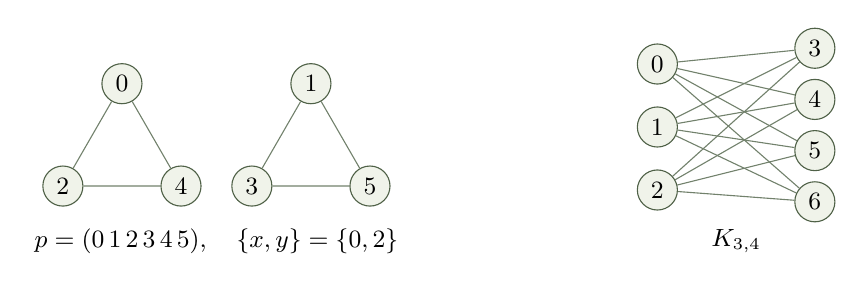
\begin{tikzpicture}[every node/.style={circle,draw=Olive,fill=PaleOlive,
  inner sep=2.5pt,font=\small},every path/.style={draw=Olive!80}]
  \node (a0) at (0,1.15) {$0$};
  \node (a2) at (-0.75,-0.15) {$2$};
  \node (a4) at (0.75,-0.15) {$4$};
  \node (a1) at (2.4,1.15) {$1$};
  \node (a3) at (1.65,-0.15) {$3$};
  \node (a5) at (3.15,-0.15) {$5$};
  \draw (a0)--(a2)--(a4)--(a0);
  \draw (a1)--(a3)--(a5)--(a1);
  \node[draw=none,fill=none,rectangle] at (1.2,-0.85)
    {$p=(0\,1\,2\,3\,4\,5),\quad\{x,y\}=\{0,2\}$};
  \begin{scope}[xshift=6.8cm]
  \foreach \i in {0,1,2} {\node (l\i) at (0,1.4-0.8*\i) {$\i$};}
  \foreach \j in {3,4,5,6} {\node (r\j) at (2.0,{1.6-0.65*(\j-3)}) {$\j$};}
  \foreach \i in {0,1,2} {\foreach \j in {3,4,5,6} {\draw (l\i)--(r\j);}}
  \node[draw=none,fill=none,rectangle] at (1,-0.85) {$K_{3,4}$};
  \end{scope}
\end{tikzpicture}
\caption{The two basic mechanisms: a same-cycle pair produces disjoint
cycles; a pair from different permutation cycles produces a bipartite graph.
These diagrams illustrate the construction, not an additional assumption.}
\label{fig:graphs}
\end{figure}

\section{First proof of nonattainment: a short qualitative
route}\label{sec:qualitative}

Before counting missing states, we prove that at least one must be missing.
The useful ingredient is a small obstruction to fitting output symmetries
into a cyclic input action.

\begin{resultbox}
\textbf{First of two independent proofs.} This section uses no counting, no
Landau function, and no refinement beyond one surjective proper base
coloring. What it buys: it is the shorter statement a referee can check
first, it is logically independent of the counting argument of
\cref{sec:quantitative}, and it is what makes the constructive algorithm of
\cref{sec:algorithm} cheap, needing only three candidate colorings instead of
the six relabelings that the counting route suggests.
\end{resultbox}

\begin{lemma}[Three relabelings cannot share a cyclic orbit]\label{lem:three}
Let $c:Q\to\D$ be surjective with $k\ge3$, and let $p$ be a permutation of
$Q$. Choose three distinct output symbols, written $0,1,2$, and let
$\sigma=(0\,1)$ and $\rho=(1\,2)$ fix all other symbols. No orbit of
precomposition by $p$ contains all three colorings
\[
 c,\qquad \sigma\circ c,\qquad \rho\circ c.
\]
\end{lemma}
\begin{proof}
Suppose one orbit contains all three. Taking $c$ as its base point, there
exist integers $r,t$ such that
\[
 \sigma\circ c=c\circ p^r,\qquad
 \rho\circ c=c\circ p^t.
\]
Using \eqref{eq:commuteactions},
\begin{align*}
 \sigma\circ\rho\circ c
 &=\sigma\circ c\circ p^t
 =c\circ p^{r+t},\\
 \rho\circ\sigma\circ c
 &=\rho\circ c\circ p^r
 =c\circ p^{t+r}.
\end{align*}
The two expressions are equal. Surjectivity of $c$ then forces
$\sigma\rho=\rho\sigma$, contrary to the chosen transpositions. For example,
they send the symbol $0$ to different symbols in the two orders.
\end{proof}

\begin{theorem}[Qualitative binary obstruction]\label{thm:qualitative}
For $3\le k\le n$ and arbitrary $a,b,\tau$, equality
\eqref{eq:fullorbit} is impossible.
\end{theorem}
\begin{proof}
If $\tau$ is not surjective, every coloring in its orbit omits at least one
of the original missing labels. Thus assume $\tau$ is surjective.

\emph{Both $a$ and $b$ are permutations.} Every orbit coloring has rank $k$,
so no constant coloring is reachable.

\emph{Both $a$ and $b$ are singular.} Choose one collision pair for each and
form a graph $H$ consisting of the resulting one or two edges. This graph is
$3$-colorable, so \cref{lem:refine} gives a proper surjective $k$-coloring.
Every nonempty product ends on the right in $a$ or $b$ and collapses the
chosen pair for that factor. Hence the only possibly reachable proper
coloring is the initial coloring $\tau$. There are at least two distinct
proper colorings, obtained by swapping two used output colors, so one is
missing.

\emph{Exactly one generator is a permutation.} Write it as $p$ and the
singular one as $s$. Choose a proper surjective coloring $c$ of
$G(p;x,y)$. All three colorings in \cref{lem:three} are proper. If every
coloring were reachable, \cref{lem:rightmost} would put all three in the
single cyclic orbit of $\tau$ under $p$. This contradicts \cref{lem:three}.
\end{proof}

The argument does not estimate the size of the transformation monoid. In
particular, merely knowing that two transformations cannot generate all of
$\TQ$ would not have sufficed: a proper submonoid could in principle still
meet every fiber of the map $t\mapsto\tau\circ t$. The graph argument
excludes this possibility directly in the output-coloring space.

\section{Second proof of nonattainment: counting the missing
colorings}\label{sec:quantitative}

\begin{resultbox}
\textbf{Second of two independent proofs.} This section proves the
quantitative inequality \eqref{eq:main}. What it buys over
\cref{sec:qualitative}: a numerical additive deficit $k!-g(k)$ valid
uniformly in $n$, which the qualitative route does not produce, and the
lemma that generalizes to arbitrary permutation groups in
\cref{prop:section}. This is the only place where the shared core theorem is
proved; every later bound refines it rather than reproving it.
\end{resultbox}

\subsection{A cyclic orbit sees only a cyclic subgroup of relabelings}

\begin{lemma}[Relabeling intersection bound]\label{lem:intersection}
Let $c:Q\to\D$ be surjective. If $O$ is any orbit under precomposition by a
permutation $p$, then
\[
 |O\cap\mathcal R(c)|\le g(k).
\]
\end{lemma}
\begin{proof}
If the intersection is empty, there is nothing to prove. Otherwise choose
$d\in O\cap\mathcal R(c)$. Then $O=\{d\circ p^j:j\in\Z\}$ and
$\mathcal R(d)=\mathcal R(c)$. Define
\[
 K=\{j\in\Z:d\circ p^j=\sigma\circ d
       \text{ for some }\sigma\in\Sym(\D)\}.
\]
For each $j\in K$, surjectivity makes $\sigma$ unique; denote it by
$\phi(j)$. We claim that $K$ is a subgroup of $\Z$ and that
$\phi:K\to\Sym(\D)$ is a homomorphism.

The exponent $0$ is in $K$. If $r,t\in K$, then
\[
 d\circ p^{r+t}
 =\phi(r)\circ d\circ p^t
 =\phi(r)\circ\phi(t)\circ d.
\]
Hence $r+t\in K$ and $\phi(r+t)=\phi(r)\phi(t)$. Also,
$d\circ p^r=\phi(r)\circ d$ implies
$d\circ p^{-r}=\phi(r)^{-1}\circ d$, so $-r\in K$.

Every subgroup of $\Z$ is cyclic. Its image $\phi(K)$ is therefore a cyclic
subgroup of $\Sym(\D)$ and has at most $g(k)$ elements. The colorings of
$O\cap\mathcal R(d)$ correspond one-to-one to these image elements. Thus
the desired intersection has size at most $g(k)$.
\end{proof}

The statement is about distinct output relabelings, not about the number of
exponents realizing them. Many powers of $p$ may induce the same coloring.
This is why the argument uses the image of a subgroup rather than the order
of $p$ itself.

It is convenient to name the cyclic orbit of an arbitrary output map:
\begin{equation}\label{eq:orbnotation}
 \Orb_\tau=\{\tau\circ p^j:j\in\Z\}.
\end{equation}
With this notation \cref{lem:intersection} reads
$|\Orb_\tau\cap\mathcal R(c)|\le g(k)$ for every surjective $c$.

\begin{remark}[A second packaging of the same bound: the setwise
stabilizer]\label{rem:setwise}
The same inequality can be obtained inside the finite cyclic group
$A=\langle p\rangle$ rather than inside $\Z$. Take $\tau=c$ first. The
nonempty fibers of $c$ form an unordered partition
$\mathcal B_c=\{c^{-1}(d):d\in\D\}$. Let $H\le A$ be its \emph{setwise}
stabilizer: those elements of $A$ that permute the blocks, without
necessarily preserving each block individually. For $h\in H$ there is a
unique $\rho(h)\in\Sym(\D)$ with
\begin{equation}\label{eq:rho}
 c\circ h=\rho(h)\circ c,
\end{equation}
uniqueness coming from surjectivity of $c$; conversely any $h\in A$
satisfying \eqref{eq:rho} for some color permutation lies in $H$. The same
composition computation as above makes $\rho:H\to\Sym(\D)$ a homomorphism,
and $|\Orb_c\cap\mathcal R(c)|=|\rho(H)|$. A subgroup of a cyclic group is
cyclic, so $\rho(H)$ is a cyclic subgroup of $\Sym(\D)$ and has at most
$g(k)$ elements. For general $\tau$, if the intersection is nonempty choose
$c'=\pi_0\circ c$ in it; then $\Orb_\tau=\Orb_{c'}$, and relabeling by
$\pi_0$ bijects $\Orb_c$ with $\Orb_{c'}$ while mapping $\mathcal R(c)$ onto
itself, so the two intersections have equal size.

What this packaging buys over \cref{lem:intersection}: it is the form that
generalizes verbatim to an arbitrary permutation group in
\cref{prop:section}, and it is the form whose characteristic failure mode
(the partition is stabilized setwise, not block by block) is flagged in
\cref{app:audit}. The $\Z$-version is kept as the working lemma because
choosing the base point $d$ inside the intersection absorbs the reduction
from a general $\tau$ that the finite-group version has to perform
separately. The two are the same mathematics in different dress, and the
different dress does different work.
\end{remark}

\begin{lemma}\label{lem:strict}
For $k\ge3$, $g(k)<k!$.
\end{lemma}
\begin{proof}
A permutation of order $k!$ would generate a cyclic subgroup of the same
size as $\Sym(\D)$, hence all of it. But $\Sym(\D)$ is not cyclic for
$k\ge3$: the transpositions of the first two and of the last two of three
distinct symbols do not commute.
\end{proof}

\subsection{Proof of the quantitative theorem}

\begin{proof}[Proof of \cref{thm:main}]
We bound the number of missing colorings in each case.

If $\tau$ is not surjective, choose any surjective coloring $c:Q\to\D$.
All $k!$ members of $\mathcal R(c)$ are absent from $\tau\langle a,b\rangle$.

Suppose $\tau$ is surjective and both generators are permutations. Choose a
coloring $c$ using exactly $k-1$ labels. None of its relabelings is reachable,
since rank is preserved. Its stabilizer in $\Sym(\D)$ is trivial: a
permutation fixing the $k-1$ used symbols must fix the one remaining symbol
as well. Thus again at least $k!$ colorings are missing.

If both generators are singular, use the graph $H$ from the qualitative
proof and a proper surjective coloring $c$. All $k!$ colorings in
$\mathcal R(c)$ are proper, but at most the initial coloring $\tau$ is
reachable. Hence at least $k!-1$ are missing.

Finally, in the mixed case choose a proper surjective coloring $c$ of the
collision-orbit graph. Its $k!$ relabelings are proper. By
\cref{lem:rightmost,lem:intersection}, at most $g(k)$ of them belong to the
reachable set. At least $k!-g(k)$ are therefore missing.

Every case gives at least $k!-g(k)$ missing colorings, since $g(k)\ge1$.
This proves the first inequality in \eqref{eq:main}. The strict inequality
is \cref{lem:strict}. Applying the reversal construction proves the automata
assertion.
\end{proof}

\begin{table}[htbp]
\centering
\begin{tabular}{@{}rrrr@{}}
\toprule
$k$ & $k!$ & $g(k)$ & Guaranteed missing colorings $k!-g(k)$\\
\midrule
3 & 6 & 3 & 3\\
4 & 24 & 4 & 20\\
5 & 120 & 6 & 114\\
6 & 720 & 6 & 714\\
7 & 5\,040 & 12 & 5\,028\\
8 & 40\,320 & 15 & 40\,305\\
9 & 362\,880 & 20 & 362\,860\\
10 & 3\,628\,800 & 30 & 3\,628\,770\\
\bottomrule
\end{tabular}
\caption{An additive deficit valid for every $n\ge k$, computed exactly from
\eqref{eq:partitions}. It is not asserted to be the optimal deficit except
at $(n,k)=(3,3)$. The accompanying file
\texttt{results/landau\_gaps.json} continues the table to $k=12$, where
$g(11)=30$ with deficit $39\,916\,770$ and $g(12)=60$ with deficit
$479\,001\,540$.}
\label{tab:landau}
\end{table}

The universal gap is deliberately simple rather than usually sharp. It
ignores all but one relabeling orbit of proper colorings. Counting the entire
proper-coloring set will give substantially stronger bounds in
\cref{sec:structural}.

\begin{remark}[Why three output labels matter]\label{rem:whythree}
For two colors the counting deficit vanishes, since $g(2)=2!=2$. Independently,
some collision-orbit graphs are odd cycles and have no proper $2$-coloring.
Both halves of the obstruction genuinely change at three colors. This is not
a hidden argument that would incorrectly prohibit binary-alphabet reversal
witnesses for ordinary languages; \cref{sec:kis2} exhibits a $k=2$ machine
reaching all $2^n$ colorings.
\end{remark}

Finally, a caution about what has been bounded. The proof does not classify
two-generated monoids, estimate their orders, or enumerate their elements.
Its bound concerns the action on output maps, which may be substantially
smaller than the monoid itself. The distinction is especially relevant when
$k<n$, where different transformations can have exactly the same composition
with $\tau$.

\section{Constructing a missing reversal state}\label{sec:algorithm}

The qualitative proof yields a useful algorithm. Its input is two explicit
transition arrays and an output array. Its output is a particular coloring
that cannot be a reversal state, together with a short explanation that can
be checked without exploring all $k^n$ colorings.

\subsection{The case split}

If an output label does not occur in $\tau$, return the constant coloring
with that label. If both letters are permutations, every reachable coloring
has the same number of occurrences of each label as $\tau$, so any constant
coloring with a different label-count vector is unreachable; deterministically,
return the constant zero coloring, unless $\tau$ is already constantly zero,
in which case return the constant one coloring.

If both letters are singular, find one collision pair for each. Properly
color their one- or two-edge graph, split classes until $k$ labels are used,
and choose this coloring unless it equals $\tau$. In that exceptional case,
swap two output labels. The resulting proper coloring is not the initial
state, and no nonempty word can reach it.

In the mixed case, form $G(p;x,y)$ by iterating the unordered pair under $p$.
At most $\binom n2$ different pairs can occur, so the graph is built in
polynomial time even when $p$ has very large order. Construct a proper
surjective coloring $c$: try a bipartite coloring first, and if the graph is
not bipartite, the proof of \cref{lem:threecolor} shows that every nonisolated
component is a cycle and every vertex has degree at most two, so greedy
coloring uses at most three colors. Then consider
\[
 c_0=c,\qquad c_1=(0\,1)\circ c,\qquad c_2=(1\,2)\circ c.
\]
Test these colorings for membership in the cyclic orbit of $\tau$. At least
one test must fail by \cref{lem:three}. Since each candidate is proper, a
failed cyclic-orbit test certifies that it is unreachable by any word.

\begin{remark}[The counting route gives a six-candidate variant]
\label{rem:sixtests}
If one starts instead from \cref{lem:intersection} rather than from
\cref{lem:three}, the natural search tests all six relabelings of a proper
coloring that uses exactly the three labels $0,1,2$: at most $g(3)=3$ of them
can lie in $\Orb_\tau$, so at most six tests are needed. More explicitly, if
$\im(\tau)$ is not exactly $\{0,1,2\}$ then the cyclic orbit contains none of
the six, and otherwise the lemma applies directly. Both variants are
implemented and both are correct; the three-candidate version is the cheaper
one, and it is available only because \cref{sec:qualitative} was proved
separately. This is one concrete payoff of keeping the two proofs apart.
\end{remark}

The only potentially nontrivial computational issue is deciding
\begin{equation}\label{eq:orbitmembership}
 c=\tau\circ p^j\quad\text{for some integer }j
\end{equation}
without iterating through all powers of $p$. The next construction resolves
it with modular arithmetic.

\subsection{A rotation constraint for each permutation cycle}

Decompose $p$ into cycles. For one cycle
\[
 C=(q_0,q_1,\ldots,q_{m-1}),\qquad p(q_i)=q_{i+1\bmod m},
\]
form the two cyclic words
\[
 U_i=\tau(q_i),\qquad V_i=c(q_i).
\]
Equation \eqref{eq:orbitmembership} requires
\[
 V_i=U_{i+j\bmod m}\qquad(0\le i<m).
\]
If $V$ is not a cyclic rotation of $U$, the candidate is immediately rejected.
Otherwise find one working shift $r$, and let $d$ be the least positive
cyclic period of $U$:
\[
 U_{i+d\bmod m}=U_i\quad\text{for all }i.
\]
Here $d\mid m$. Every working shift satisfies exactly the congruence
\begin{equation}\label{eq:shiftcongruence}
 j\equiv r\pmod d.
\end{equation}

\begin{lemma}\label{lem:shiftcoset}
The shifts fixing a cyclic word of length $m$ form a subgroup of
$\Z/m\Z$. If a target word is one rotation of the source, the shifts taking
the source to the target form a coset of this subgroup. Equivalently, they
are precisely one residue class modulo the least cyclic period.
\end{lemma}
\begin{proof}
The identity shift fixes the word; the composition and inverse of fixing
shifts also fix it. Thus the fixing shifts form a subgroup. If $r$ takes the
source to the target, another shift $j$ does so exactly when $j-r$ fixes the
source. Subgroups of $\Z/m\Z$ consist of the multiples of a divisor of $m$,
and the least positive period is that divisor.
\end{proof}

For example, the word $010101$ has least cyclic period $2$, not $6$.
A target $101010$ contributes the constraint $j\equiv1\pmod2$. Using the
whole cycle length as the modulus would incorrectly discard valid shifts.

\subsection{Combining the constraints}

Maintain a congruence $j\equiv R\pmod M$, initially $R=0$, $M=1$.
To add $j\equiv r\pmod d$, put $g=\gcd(M,d)$. The two congruences are
compatible if and only if
\[
 r-R\equiv0\pmod g.
\]
When they are compatible, write $j=R+Mt$. Dividing by $g$ gives
\[
 \frac{M}{g}t\equiv\frac{r-R}{g}\pmod{d/g}.
\]
The coefficient $M/g$ is invertible modulo $d/g$, so this determines a unique
class of $t$ and hence one class of $j$ modulo $\lcm(M,d)$. Modulus $1$ is
handled as a vacuous congruence.

A rejection certificate is either a cycle whose target is not a rotation of
the source, or a pair of incompatible accumulated congruences. A successful
test returns an exponent representing the solution class. At most three such
tests are needed to produce an unreachable proper coloring.

\subsection{A second, deliberately different membership
criterion}\label{sec:crtpairwise}

The incremental merge just described is not the only way to decide the
system. Suppose the cycles contribute congruences
$j\equiv r_i\pmod{p_i}$ for $i=1,\ldots,\nu$. The generalized Chinese
remainder theorem says that the system is solvable exactly when every pair is
compatible:
\begin{equation}\label{eq:crtcompat}
 r_i\equiv r_{i'}\pmod{\gcd(p_i,p_{i'})}\qquad\text{for all }i,i'.
\end{equation}
Sufficiency follows by prime powers. For each prime, select a congruence
whose modulus carries the largest exponent of that prime. Pairwise
compatibility makes its residue agree with every weaker requirement at that
prime. The selected prime-power congruences have coprime moduli and combine
by the ordinary Chinese remainder theorem, and their common solution
satisfies the original system.

What this buys over the incremental merge: nothing mathematically, and that
is the point. The two criteria are used by two programs that share no code,
so a disagreement between them exposes an implementation mistake in one of
them. The producer \texttt{code/dfao.py} merges congruences iteratively; the
standalone verifier \texttt{code/certificate\_checker.py} uses
\eqref{eq:crtcompat}. This deliberate divergence of method is the substance
of the trust separation described in \cref{sec:trust}, and the two
implementations are not unified.

\begin{proposition}[Polynomial-time constructive obstruction]\label{prop:algorithm}
For explicit arrays $a,b,\tau$ with $3\le k\le n$, one can construct a
coloring outside $\tau\langle a,b\rangle$ in time polynomial in the input
size, without enumerating the coloring orbit or the transformation monoid.
The construction also admits a polynomial-size certificate that can be
checked in polynomial time.
\end{proposition}
\begin{proof}
Finding collisions and decomposing a permutation into cycles are elementary
finite-array operations. The graph has at most $\binom n2$ edges and can be
built in polynomial time. It is either bipartite or has maximum degree at
most two, so the initial proper coloring is obtained by a breadth-first
bipartite coloring or a greedy $3$-coloring. Splitting color classes takes at
most $k$ further steps.

The simple implementation tests all rotations of each cycle word, requiring
$O(\sum m_i^2)\le O(n^2)$ symbol comparisons for one cyclic-orbit test.
The least periods can be found within the same bound. The moduli in the
Chinese remainder calculation divide $\lcm(1,2,\ldots,n)$ and therefore
have at most $O(n\log n)$ bits, using the elementary bound by $n!$.
Euclidean arithmetic and modular inverses on these integers take polynomial
time. Only three candidate tests are needed.

For the certificate clause, a certificate consists of the input arrays and
the target, together with either a differing label-count vector, or two
collision pairs, or one collision pair with its orbital graph and evidence of
cyclic nonmembership. In the last case the evidence is a cycle whose target
word is no rotation of the source word, or a pair of incompatible period
congruences; a checker may instead recompute all congruences and reject
membership directly. The graph has at most $\binom n2$ edges and every tuple
has length at most $n$, so both the certificate size and the checking time
are polynomial.
\end{proof}

\subsection{A concrete certificate}

Consider the $8$-state, $5$-output machine whose arrays are
\begin{align*}
 p&=(1,2,0,4,5,6,7,3),\\
 s&=(3,2,1,3,4,5,6,0),\\
 \tau&=(0,1,2,3,4,4,4,4).
\end{align*}
Array notation means, for example, $p(0)=1$. The collision $s(0)=s(3)$
generates $K_{3,5}$ between $\{0,1,2\}$ and $\{3,4,5,6,7\}$.
The algorithm returns
\[
 c=(2,3,0,4,1,1,1,1).
\]
Its two block palettes, $\{0,2,3\}$ and $\{1,4\}$, are disjoint, so it is
proper. On the first cycle, however, $(2,3,0)$ is not a rotation of the
source word $(0,1,2)$. Thus $c$ is not a power-rotation of $\tau$, and no word
containing $s$ can reach a proper coloring. This proves that $c$ is missing.
The full machine-readable certificate is in
\texttt{data/example\_certificate.json}. Its schema is
\begin{multline*}
 \{n,k,a,b,\tau,\ \texttt{unreachable}\{\texttt{case},\texttt{target},
 \texttt{permutation},\texttt{singular},\\
 \texttt{collision},\texttt{edges},\texttt{candidate\_tests}[\ldots]\}\},
\end{multline*}
recording the $15$ edges of $K_{3,5}$ and, for each of the three candidates,
the outcome of its cyclic-orbit test with reason \texttt{nonrotation}.

\subsection{Two certificate formats and two
generators}\label{sec:twocerts}

The archive ships a second, differently shaped certificate family, produced
by a different search and validated by a different program. Its schema is
\[
 \{n,k,a,b,\tau,\texttt{case},\texttt{permutation\_letter},\texttt{pair},
 \texttt{edges},\texttt{target},
 \texttt{cyclic\_nonmembership}\{\ldots\}\},
\]
in \texttt{results/certificates.json}, where the nonmembership block records
\texttt{member}, \texttt{reason}, \texttt{cycle} and \texttt{constraints}.
Four such certificates are supplied, all in the one-permutation case: at
$(n,k)=(3,3)$ with target $[0,2,1]$; at $(4,3)$ and $(4,4)$ with target
$[2,1,0,1]$; and at $(5,3)$ with target $[2,0,1,1,1]$. All four carry the
reason \texttt{no\_rotation}.

The two formats are kept side by side and neither schema is normalized onto
the other. What each buys: the \texttt{results/certificates.json} family is
produced by the six-relabeling search of \cref{rem:sixtests} and is checked
by the import-free verifier described below, which is what makes it useful
as a trust artifact, and its structural variant scales to $n\le50$ without
any orbit enumeration; the \texttt{data/example\_certificate.json} family is
produced by the three-candidate search driven by \cref{lem:three}, records
the candidate-by-candidate test log that the cheaper search generates, and
describes a single large machine, the $8$-state, $5$-output $K_{3,5}$
example whose orbit is computed exactly in \cref{sec:finite}. Different
search strategies and different scales make agreement between them
informative.

\subsection{Implementation and trust separation}\label{sec:trust}

The file \texttt{code/dfao.py} constructs the certificates of the first
family. The separate file
\texttt{code/\allowbreak certificate\_\allowbreak checker.py} imports no
code from that module. It recomputes the collision conditions, the entire
pair orbit, properness, and cyclic nonmembership, using the pairwise
criterion \eqref{eq:crtcompat} rather than the producer's iterative merge,
and exits with a nonzero status if any supplied certificate is rejected.

This independence is limited, and is stated precisely. Both programs
implement the same mathematical argument, so they are not an independent
proof of the theorem. They are independent checks of finite certificates
under that argument. The archive also includes randomized comparisons with
explicit cyclic-orbit enumeration and direct comparisons with complete
reverse-state searches.

\section{Why three input letters suffice}\label{sec:ternary}

The binary obstruction is an exact alphabet-size threshold, not an
obstruction to maximal reversal in general. We include a construction to
make this distinction explicit.

\begin{theorem}[Ternary attainability]\label{thm:ternary}
For every $3\le k\le n$, some minimal $n$-state DFAO with three input letters
and $k$ output values has reversal state complexity $k^n$.
\end{theorem}
\begin{proof}
Let $Q=\{0,\ldots,n-1\}$. Use three transformations:
\[
 p=(0\,1\,\cdots\,n-1),\qquad t=(0\,1),
\]
and the map $e$ that sends $1$ to $0$ and fixes every other point.
Conjugating $t$ by powers of $p$ yields the adjacent transpositions, so $p$
and $t$ generate $\Sym(Q)$.

Conjugates of $e$ by permutations give every elementary collapse that sends
one chosen point to another and fixes all remaining points. These collapses
and the permutations generate every transformation of $Q$. To see this,
let $f:Q\to Q$ be arbitrary. Choose one representative $r_y\in f^{-1}(y)$
for each $y\in\im(f)$. Collapse every other point of $f^{-1}(y)$ onto $r_y$.
The resulting transformation $h$ satisfies $h(q)=r_{f(q)}$. The bijection
$r_y\mapsto y$ between two equally sized subsets extends to a permutation
$u$ of $Q$. Then $f=u\circ h$.

Choose any surjective output map $\tau:Q\to\D$. Given any coloring
$c:Q\to\D$, choose a representative $r_d\in\tau^{-1}(d)$ for every output
symbol $d$, and define $f_c(q)=r_{c(q)}$. Then $\tau\circ f_c=c$.
Since the transition monoid is all of $\TQ$, every coloring is reachable in
the reversal construction. The original machine is accessible because it
contains the $n$-cycle $p$. Hence \cref{prop:orbit} gives $k^n$ distinguishable
reversal states.

The original machine is also minimal. If $q\ne q'$, choose states $u,v$
with different outputs. A transformation sending $q$ to $u$ and $q'$ to $v$
is realized by an input word, which distinguishes $q$ from $q'$.
\end{proof}

Combining this theorem with \cref{thm:main} proves the second assertion of
\cref{cor:sc}: the least input-alphabet size that permits all $k^n$ reversal
states is exactly three for $3\le k\le n$. A one-letter machine is covered by
duplicating its transformation.

\begin{remark}[The two-value case]\label{rem:ternary-two}
One of the two source reports stated this attainability for every $n\ge k\ge2$.
Its construction uses only that $p$ and $t$ generate $\mathrm{Sym}(Q)$ and that
elementary mergers together with permutations generate all of $T(Q)$, neither
of which needs $k\ge3$, so the case $k=2$ is covered on the same grounds. The
deficit of \cref{thm:main} is a separate matter and is claimed only for
$k\ge3$.
\end{remark}

Ternary attainability was already established
in the target paper \cite[Theorem~1 and Corollary~2]{Davies2017}; the
verification above only fixes conventions, and the new obstruction supplies
the missing binary exclusion.

\subsection{Why two output values are different}\label{sec:kis2}

The proof genuinely needs three output values. A collision-orbit graph can
contain an odd cycle and then has no proper $2$-coloring. Independently,
$\Sym(\{0,1\})$ is cyclic, so the noncommuting-relabellings argument is
unavailable even when a proper binary coloring exists.

A small explicit example uses
\[
 p=(1,2,0),\qquad s=(0,0,2),\qquad\tau=(0,0,1).
\]
The orbit contains all eight binary colorings of three states. Powers of $p$
provide the three colorings with one $1$. Applying $s$ to a suitable one
provides a coloring with two $1$s, whose rotations give the other two.
The same collapse produces $000$ from a one-$1$ coloring and $111$ from a
two-$1$ coloring. Thus the small example already shows that the conclusion
cannot simply be extended to $k=2$.

The cases $k=1$ and $k>n$ are outside the interesting range. The former gives
a constant function; in the latter, no output map can use all $k$ labels,
and missing output values already prevent a full coloring orbit.

\section{An extension to abelian permutation groups}\label{sec:abelian}

The cyclic nature of the single permutation letter can be weakened. The
same mechanism applies to any number of commuting permutation letters,
provided there is only one singular letter.

\subsection{The group-theoretic form of the intersection lemma}

\begin{proposition}[Relabelings induced by a permutation group]\label{prop:section}
Let $H\le\Sym(Q)$ and let $c:Q\to\D$ be surjective. If $O$ is an $H$-orbit
of colorings, then the nonempty intersection $O\cap\mathcal R(c)$ has size
$|J|$ for a subgroup $J\le\Sym(\D)$ that is a homomorphic image of a subgroup
of $H$.
\end{proposition}
\begin{proof}
Choose $d\in O\cap\mathcal R(c)$, so $O=dH$ and
$\mathcal R(d)=\mathcal R(c)$. Define
\[
 K=\{h\in H:d\circ h=\sigma\circ d
                \text{ for some }\sigma\in\Sym(\D)\}.
\]
The output permutation is unique. The same composition and inverse
calculation as in \cref{lem:intersection} shows that $K$ is a subgroup of
$H$ and that the assignment $h\mapsto\sigma$ is a homomorphism. Its image
$J$ parametrizes exactly the colorings in the intersection.
\end{proof}

Thus a full output-relabeling orbit would force $\Sym(\D)$ to be a quotient
of a subgroup of $H$. This is a general obstruction, although the graph
colorability condition must still be checked.

\begin{remark}[Several singular generators]\label{rem:severalsingular}
Nothing above needs a single singular letter. Let $H\le\Sym(Q)$ be generated
by any set of permutation letters, let $b_1,\ldots,b_r$ be singular
letters, and choose one collision pair $e_i$ for each $b_i$. Put
\begin{equation}\label{eq:generalgraph}
 E=\bigcup_{i=1}^{r}\{h(e_i):h\in H\}.
\end{equation}
A composition containing a singular letter has a rightmost such letter and a
suffix in $H$, so exactly as in \cref{lem:rightmost} its output coloring is
improper for this graph, and the reachable proper colorings lie in $\tau H$.
If that graph has a proper surjective $k$-coloring $c$, taking $H$ to be the
setwise stabilizer of the fiber partition of $c$ as in \cref{rem:setwise}
shows that full reachability forces $\rho(H)=\Sym(\D)$.

The colorability hypothesis cannot simply be dropped. With many collision
pairs or a large permutation group, the graph of \eqref{eq:generalgraph} can
require more than $k$ colors. Moreover, a nonabelian permutation group can
genuinely have a symmetric-group quotient. These two escape routes are
exactly why the extension does not contradict the three-letter
full-transformation witness of \cref{thm:ternary}.
\end{remark}

\subsection{Orbit graphs for abelian groups}

For a collision pair $s(x)=s(y)$, define
\[
 E(G_H)=\{\{h(x),h(y)\}:h\in H\}.
\]
A word containing $s$ can again be written $u\circ s\circ h$ with $h\in H$.
It collapses an edge of $G_H$, so reachable proper colorings must lie in the
single $H$-orbit $\tau H$.

\begin{lemma}\label{lem:abeliangraph}
If $H$ is abelian, the graph $G_H$ is $3$-colorable.
\end{lemma}
\begin{proof}
If $x$ and $y$ lie in different $H$-orbits, all edges join those two orbits,
so the graph is bipartite. Otherwise write $y=h_0(x)$ for some $h_0\in H$.
For a vertex $z=h(x)$, commutativity gives
\[
 h(y)=h(h_0(x))=h_0(h(x))=h_0(z).
\]
Thus the edges on the orbit of $x$ are exactly $\{z,h_0(z)\}$. Every vertex
has at most two neighbors. All other vertices are isolated, so three colors
suffice.
\end{proof}

Let $A(k)$ denote the largest order of an abelian subgroup of $\Sym(k)$.
There is a simple exact expression:
\begin{equation}\label{eq:abelianmax}
 A(k)=\max_{\lambda\vdash k}\prod_i\lambda_i.
\end{equation}
To prove the upper bound, decompose an abelian permutation group into its
orbits of sizes $\lambda_i$. On one orbit, an element fixing one point fixes
every point, because it commutes with the transitive action. The faithful
image on that orbit is therefore regular, of order $\lambda_i$. The original
group embeds into the product of these images, so its order is at most
$\prod_i\lambda_i$. Conversely, disjoint cyclic groups of orders
$\lambda_i$ attain that product.

For $k\ge2$, the usual elementary product maximization gives
\[
 A(k)=
 \begin{cases}
 3^{k/3},&k\equiv0\pmod3,\\
 4\cdot3^{(k-4)/3},&k\equiv1\pmod3,\ k\ge4,\\
 2\cdot3^{(k-2)/3},&k\equiv2\pmod3.
 \end{cases}
\]
Indeed, a part at least $5$ is improved by replacing it with $3$ and the
remaining part; parts $1$ are eliminated in a maximizing partition for
$k\ge2$; and three parts $2$ are improved by two parts $3$. A leftover $4$
may be kept as $4$ or split into $2+2$.

\begin{theorem}[Abelian-permutation obstruction]\label{thm:abelian}
Let $H\le\Sym(Q)$ be abelian, let $s:Q\to Q$ be singular, and let
$3\le k\le n$. Then, for every $\tau:Q\to\D$,
\[
 |\tau\langle H,s\rangle|\le k^n-k!+A(k)<k^n.
\]
\end{theorem}
\begin{proof}
A nonsurjective $\tau$ omits all $k!$ relabelings of any surjective coloring.
Otherwise, \cref{lem:abeliangraph,lem:refine} gives a proper surjective
$k$-coloring of $G_H$. Its reachable relabelings must lie in $\tau H$.
By \cref{prop:section}, those relabelings form a set whose size is the order
of an abelian subgroup of $\Sym(\D)$, and so is at most $A(k)$. The remaining
$k!-A(k)$ relabelings are missing. Since $\Sym(k)$ is nonabelian for $k\ge3$,
$A(k)<k!$.
\end{proof}

This does not forbid three-letter maximal examples in general: the two
permutation letters in \cref{thm:ternary} generate a nonabelian group. It
instead identifies a structural requirement on any such construction with
one singular letter.

\section{Sharper bounds from all proper colorings}\label{sec:structural}

The graph-coloring viewpoint has antecedents in Holzer and K\"onig's work
on transformation monoids \cite[Sections~4--5]{HolzerKoenig2004}; the
coloring count is not presented here as a newly invented technique.
The factorial gap counts one free output-relabeling orbit. We now count all
proper colorings of a collision-orbit graph. The resulting bound retains
information about the cycle structure of the permutation and is often sharp.

\subsection{The basic chromatic bound}

Let $P_G(k)$ be the number of proper maps $Q\to\D$. In the mixed case,
\cref{lem:rightmost} immediately gives
\begin{equation}\label{eq:chromaticbound}
 |\tau\langle p,s\rangle|
 \le k^n-P_G(k)+\ord(p).
\end{equation}
More generally, $\ord(p)$ may be replaced by any bound on the $p$-orbit
length of a proper coloring. If $\tau$ is improper, no proper coloring is
reachable at all; using the larger term remains a valid upper bound.

Replacing $\ord(p)$ by the actual orbit size, and splitting on properness
rather than absorbing it, gives a strictly sharper statement for a given
machine.

\begin{proposition}[Chromatic deficit, instance-specific
form]\label{prop:chromatic}
Let $p$ be a permutation, let $s$ be singular, fix a collision pair
$\{x,y\}$ of $s$, and put $G=G(p;x,y)$ and $M=\langle p,s\rangle$. Then
\begin{equation}\label{eq:chromaticsharp}
 |\tau M|\le k^n-P_G(k)+
 \begin{cases}
  |\Orb_\tau|,&\tau\text{ is proper for }G,\\
  0,&\tau\text{ is not proper for }G.
 \end{cases}
\end{equation}
\end{proposition}
\begin{proof}
The permutation $p$ is a graph automorphism of $G$, since $E(G)$ was defined
in \eqref{eq:orbitgraph} as a $p$-invariant set of pairs. Its pullback
action therefore preserves properness, so the orbit $\Orb_\tau$ of
\eqref{eq:orbnotation} is wholly proper or wholly improper according to
whether $\tau$ is proper. By \cref{lem:rightmost}, every reachable proper
coloring lies in that orbit. There are $k^n-P_G(k)$ improper colorings in
total, and at most the stated number of reachable proper ones. Adding the two
counts gives \eqref{eq:chromaticsharp}.
\end{proof}

\begin{remark}[Two instance-specific chromatic bounds, and what each
buys]\label{rem:twochromatic}
Inequalities \eqref{eq:chromaticbound} and \eqref{eq:chromaticsharp} are both
kept, and neither substitutes for the other.
\Cref{prop:chromatic} is sharper for any fixed machine, because
$|\Orb_\tau|$ divides $\ord(p)$ and is usually much smaller, and because an
improper $\tau$ contributes nothing at all; it is what yields the exact
values $24$, $67$, $176$ and $215$ in \cref{sec:instances}.
Inequality \eqref{eq:chromaticbound} is weaker for a given instance but is
stated in terms of $\ord(p)$ alone, and that is precisely what allows it to
be maximized over all collision graphs without reference to $\tau$; it is the
form that abstracts into the residual-order function $H_r(t)$, the period
improvement $T_{r,k}(a,b)$, and hence the universal bound $U(n,k)$ of
\cref{thm:structural}. The instance-specific version cannot play that role,
since $|\Orb_\tau|$ is not a function of the graph parameters.
\end{remark}

Neither inequality asserts that all improper colorings are reachable. That
additional saturation property must be proved or checked separately for any
claimed equality witness, which is why a graph bound alone does not solve the
exact state-complexity optimization problem.

There are only two structural forms for $G(p;x,y)$.

\subsection{A pair in one permutation cycle}

Suppose the pair lies on a cycle of length $m$, with displacement $h$.
Put
\[
 d=\gcd(m,h),\qquad L=m/d,\qquad r=n-m.
\]
The graph consists of $d$ disjoint cycles of length $L$, together with $r$
isolated vertices. When $L=2$, each component is one edge rather than a
cycle with two parallel edges; the coloring count is unchanged.

For $L\ge2$, the appropriate cycle factor is
\begin{equation}\label{eq:cyclepoly}
 C_L(k)=(k-1)^L+(-1)^L(k-1).
\end{equation}
One direct derivation uses the $k\times k$ matrix $B$ with zeros on the
diagonal and ones elsewhere. A proper coloring of a labeled cyclic sequence
is a closed walk, so the count is $\operatorname{tr}(B^L)$. The constant
vectors have eigenvalue $k-1$, and the subspace of coordinate sum zero has
eigenvalue $-1$ and dimension $k-1$. This gives \eqref{eq:cyclepoly}. At
$L=2$ the formula is $k(k-1)$, the count for one edge.

Therefore
\begin{equation}\label{eq:samecount}
 P_G(k)=C_L(k)^d k^r.
\end{equation}
Every divisor $d\mid m$ with $d<m$ is possible: take displacement $h=d$.

\subsection{A pair in different permutation cycles}

Let the cycle lengths be $a,b$, and put
\[
 d=\gcd(a,b),\qquad u=a/d,\qquad v=b/d,\qquad r=n-a-b.
\]
Label the two cycles by $\Z/a\Z$ and $\Z/b\Z$, putting the chosen endpoints
at their respective origins. An edge joins $i$ to $j$ exactly when a common
power of $p$ carries the origin pair to $(i,j)$. The generalized Chinese
remainder criterion says this occurs precisely when
$i\equiv j\pmod d$. Hence
\[
 G\cong dK_{u,v}\ \sqcup\ rK_1.
\]

The proper-coloring count for $K_{u,v}$ is
\begin{equation}\label{eq:bipoly}
 B_k(u,v)=\sum_{i=1}^{\min(u,k)}
      \fall{k}{i}\stirling{u}{i}(k-i)^v.
\end{equation}
To derive it, let the left side use exactly $i$ colors. Partition its $u$
labeled vertices into $i$ nonempty color classes in
$\stirling{u}{i}$ ways, assign distinct output labels to the classes in
$\fall{k}{i}=k!/(k-i)!$ ways, and color each right-side vertex with one of
the remaining $k-i$ labels. Thus
\begin{equation}\label{eq:diffcount}
 P_G(k)=B_k(u,v)^d k^r.
\end{equation}
This derivation also proves the symmetry $B_k(u,v)=B_k(v,u)$, even though
\eqref{eq:bipoly} does not display it symmetrically.

For three colors the expression simplifies considerably:
\begin{equation}\label{eq:threebip}
 B_3(u,v)=3\bigl(2^u+2^v-2\bigr),\qquad u,v\ge1.
\end{equation}
Only $i=1,2$ contribute in \eqref{eq:bipoly}, and
$\stirling{u}{2}=2^{u-1}-1$.

\subsection{Choosing a collision pair}

A singular map may have many collision pairs. Each one gives a valid bound of
the form \eqref{eq:chromaticsharp}, so taking the minimum over all collision
pairs of $s$ is a legitimate improvement. Alternatively, the union of all the
corresponding orbital graphs is still a valid obstruction graph, because a
word containing $s$ collapses one of its edges whichever pair is chosen.
That union may, however, cease to be three-colorable, and its chromatic
polynomial may be harder to compute. The uniform proof deliberately uses a
single pair: that choice is what preserves the elementary
three-colorability argument of \cref{lem:threecolor} for every permutation,
and hence the guaranteed supply of surjective proper colorings.

\subsection{Worked instances}\label{sec:instances}

Tuples list map values in the order $0,1,\ldots,n-1$. All orbit counts in
this subsection are computed by exact integer-state breadth-first search.

\smallskip
\noindent\emph{Sharpness at three states and three outputs.} Take
\begin{equation}\label{eq:n3}
 a=(1,2,0),\qquad b=(0,0,2),\qquad\tau=(0,1,2).
\end{equation}
The collision pair $\{0,1\}$ produces a triangle under the three-cycle $a$.
There are six proper three-colorings, and the pure-$a$ orbit of $\tau$ is
$(0,1,2)$, $(1,2,0)$, $(2,0,1)$, of size three. Thus
\cref{prop:chromatic} gives at most $27-6+3=24$ reachable states. The word
table of \cref{app:words} exhibits $24$ distinct colorings, so this automaton
has exactly $24$ reverse states and the three missing ones are
\[
 (0,2,1),\qquad(1,0,2),\qquad(2,1,0).
\]
The original machine is accessible and minimal: the cycle reaches every
state, and $\tau$ already separates states without a continuation. Hence
equality holds in \cref{thm:main} at $n=k=3$.

\smallskip
\noindent\emph{Four-state examples.} Use $a=(1,2,3,0)$, $b=(0,0,3,2)$, again
with the collision pair $\{0,1\}$, whose orbital graph is the four-cycle
$C_4$. For three colors take $\tau=(0,1,0,2)$: it is proper, its cyclic orbit
has size four, and $C_4(3)=2^4+2=18$ by \eqref{eq:cyclepoly}, so the bound is
$81-18+4=67$. For four colors take $\tau=(0,1,2,3)$: now $C_4(4)=3^4+3=84$
and the bound is $256-84+4=176$. Exact search attains both. Both machines are
accessible and minimal.

\smallskip
\noindent\emph{A complete-bipartite example.} Let
\[
 a=(1,0,3,4,2),\qquad b=(2,1,2,3,0),\qquad\tau=(0,1,2,2,2).
\]
The permutation has cycles $(0\,1)$ and $(2\,3\,4)$, while $b$ identifies $0$
and $2$, so the orbital graph is $K_{2,3}$. By \eqref{eq:bipoly},
\[
 B_3(2,3)=3\cdot2^3+6\cdot1^3=30,
\]
in agreement with \eqref{eq:threebip}. The coloring $\tau$ is proper with
orbit size two under $a$, so \cref{prop:chromatic} gives $3^5-30+2=215$,
which the included search attains.

\begin{remark}[Two different $n=5$, $k=3$ examples]\label{rem:twofives}
The value $215$ just obtained is an \emph{instance-specific} equality for
this particular $K_{2,3}$ machine; it is not a claim that $215$ is the global
five-state, three-output maximum. \Cref{app:witnesses} lists a different
five-state machine, $p=(1,2,3,4,0)$, $s=(0,0,3,4,2)$, $\tau=(0,1,0,1,2)$,
whose orbit has size $218=U(5,3)$ and which realizes the small-case maximum
of \cref{sec:finite}. The two examples illustrate different claims, the first
that the cross-cycle formula is exactly attained and the second that the
structural bound is met, and $215<218$ is a consequence of the first machine
not being extremal. They are not in conflict, and neither replaces the other.
\end{remark}

\begin{table}[htbp]
\centering
\begin{tabular}{@{}rrrrrr@{}}
\toprule
$n$ & $k$ & $k^n$ & Uniform bound & Graph bound & Actual witness orbit\\
\midrule
3 & 3 & 27 & 24 & 24 & 24\\
4 & 3 & 81 & 78 & 67 & 67\\
4 & 4 & 256 & 236 & 176 & 176\\
5 & 3 & 243 & 240 & 215 & 215\\
\bottomrule
\end{tabular}
\caption{The uniform estimate of \cref{thm:main} is designed to prove
nonattainment; the instance-specific graph estimate of \cref{prop:chromatic}
can be much stronger for a particular pair of generators. The last row is the
$K_{2,3}$ machine of \cref{rem:twofives}, not the extremal five-state one.}
\label{tab:examples}
\end{table}

The values $24$, $67$ and $176$ are not new numerical records: they occur
among the previously verified maxima in \cite[Table~3]{Davies2017}. Here they
serve as independent regression tests and as examples where the collision
graph explains the missing states. For every example the archive records the
input maps, the exact orbit size, a minimality check, and an explicit
unreachable coloring; the certificate checker verifies nonreachability
structurally, without relying on the breadth-first search that produced the
orbit counts.

\subsection{Accounting for the remaining permutation cycles}

Let $\mathcal O_r$ be the set of orders of permutations on $r$ points,
with $\mathcal O_0=\{1\}$. Define
\begin{equation}\label{eq:H}
 H_r(t)=\max_{o\in\mathcal O_r}\lcm(t,o).
\end{equation}
For a same-cycle pair the distinguished cycle contributes order $m$, so
\[
 \ord(p)\le H_r(m).
\]
For a different-cycle pair, the two distinguished cycles contribute
$\lcm(a,b)$, giving
\[
 \ord(p)\le H_r(\lcm(a,b)).
\]
The exact set of possible residual orders matters. In general one must not
replace $H_r(t)$ by $\lcm(t,g(r))$: the residual order maximizing an ordinary
integer magnitude need not maximize its least common multiple with $t$.

For example, $g(5)=6$. If $t=6$, then $\lcm(t,g(5))=6$, whereas a residual
$5$-cycle gives $\lcm(6,5)=30$. The definition \eqref{eq:H} handles such
interactions correctly.

\subsection{The three-color period improvement}

When $k=3$ and $\gcd(a,b)=1$, the nonisolated part is the connected graph
$K_{a,b}$. In a proper coloring the palettes on the two sides are disjoint.
Since only three labels are available and both palettes are nonempty, at
least one side is monochromatic. Its rotation contributes period $1$.
Thus the proper-coloring period on the two distinguished cycles divides
$a$ or divides $b$, rather than necessarily requiring $\lcm(a,b)$.
Including the isolated vertices gives the improved bound
\begin{equation}\label{eq:periodimprove}
 T_{r,k}(a,b)=
 \begin{cases}
 \max\{H_r(a),H_r(b)\},&k=3,\ \gcd(a,b)=1,\\
 H_r(\lcm(a,b)),&\text{otherwise}.
 \end{cases}
\end{equation}
The connectedness condition is important. We do not apply the improvement
component by component when $\gcd(a,b)>1$, because the permutation may rotate
the components as well as the colors within them.

\subsection{A universal finite formula}

The two unmixed generator cases also admit easy bounds. If both letters
are permutations, the orbit lies in one fixed color histogram. The largest
possible histogram class is the balanced multinomial coefficient
\[
 M(n,k)=\frac{n!}{(q!)^{k-z}((q+1)!)^z},\qquad n=qk+z,\quad0\le z<k.
\]
Balancing is optimal because replacing two counts $a\ge b+2$ by $a-1,b+1$
decreases the product of their factorials.

If both letters are singular, their two chosen collision edges have at
least $(k-1)^2k^{n-2}$ proper colorings. For two distinct edges the count is
exactly this whether they share a vertex or are disjoint; for a repeated
edge the count is larger. At most the initial coloring is reachable among
them. Thus the missing-coloring count is at least
\[
 (k-1)^2k^{n-2}-1.
\]

Define $D(n,k)$ to be the minimum of the following finite collection:
\begin{align}
 &k^n-(k-1)^n,\label{eq:Dnon}\\
 &k^n-M(n,k),\label{eq:Dperm}\\
 &(k-1)^2k^{n-2}-1,\label{eq:Dsing}\\
 &C_{m/d}(k)^d k^{n-m}-H_{n-m}(m),\label{eq:Dcycle}\\
 &B_k(a/d,b/d)^d k^{n-a-b}-T_{n-a-b,k}(a,b).\label{eq:Dbip}
\end{align}
In \eqref{eq:Dcycle}, the parameters range over $2\le m\le n$ and positive
divisors $d\mid m$ with $d<m$. In \eqref{eq:Dbip}, they range over
$1\le a\le b$, $a+b\le n$, with $d=\gcd(a,b)$.
The first entry handles nonsurjective output maps. It is unnecessary when
surjectivity is part of the definition of the extremal problem, but makes
the bound valid for arbitrary supplied output arrays.

\begin{theorem}[Structural upper bound]\label{thm:structural}
For every $3\le k\le n$ and arbitrary $a,b,\tau$,
\begin{equation}\label{eq:structural}
 |\tau\langle a,b\rangle|\le U(n,k):=k^n-D(n,k).
\end{equation}
It is always valid to combine this with \cref{thm:main} by taking the smaller
of $U(n,k)$ and $k^n-k!+g(k)$.
\end{theorem}
\begin{proof}
Every machine belongs to one of the nonsurjective, two-permutation,
two-singular, or mixed cases. The first three give
\eqref{eq:Dnon}--\eqref{eq:Dsing}. In the mixed case choose any collision pair.
If its endpoints are on the same permutation cycle, use
\eqref{eq:samecount} and the order bound $H_{n-m}(m)$. Otherwise use
\eqref{eq:diffcount} and \eqref{eq:periodimprove}. These are exactly the
entries \eqref{eq:Dcycle} and \eqref{eq:Dbip}. The actual machine therefore
misses at least one entry of this collection, and hence at least its minimum.
\end{proof}

The bound is obtained without enumerating transformations. There are only
quadratically many choices of the displayed graph parameters up to divisor
bookkeeping. Computing the residual order sets involves integer partitions;
we do not claim that this part is a polynomial-time algorithm in $n$.
It is nevertheless a much smaller exact computation than enumerating all
$n^{2n}$ ordered pairs of transformations, let alone their output orbits.

\section{Finite optimality results and explicit witnesses}\label{sec:finite}

\subsection{Comparison with the published lower bound}

For $3\le k<n$, define
\begin{equation}\label{eq:lower}
 L(n,k)=\max_{\substack{1<\ell<m,\ \ell+m=n\\\gcd(\ell,m)=1}}
 \bigl[k^n-B_k(\ell,m)+G_k(\ell,m)\bigr],
\end{equation}
where
\[
 G_k(\ell,m)=
 \begin{cases}
 m,&k=3,\\
 \ell m,&k\ge4.
 \end{cases}
\]
Davies's Corollary~3 provides accessible binary DFAO witnesses attaining
this lower bound \cite{Davies2017}. We use that result as a literature
dependency for the finite optimality comparison, not for the principal
obstruction theorem.

Let $R_2(n,k)$ denote the largest reversal complexity of an accessible
$n$-state binary DFAO using $k$ output values. Then
\[
 L(n,k)\le R_2(n,k)\le U(n,k).
\]
For the displayed range $n\ge7$, admissible coprime splits always exist.
For example, take the neighboring halves for odd $n$; for $n\equiv0\pmod4$
take $n/2-1,n/2+1$; and for $n\equiv2\pmod4$, $n\ge10$, take
$n/2-2,n/2+2$.

\begin{proposition}[Computer-assisted finite equality]\label{prop:finite}
Exact evaluation of \eqref{eq:lower} and \eqref{eq:structural} gives
\[
 L(n,k)=U(n,k)
 \qquad(7\le n\le30,\ 3\le k<n).
\]
Consequently these values equal $R_2(n,k)$ throughout that finite range.
There are $\sum_{n=7}^{30}(n-3)=372$ parameter pairs.
\end{proposition}

The complete exact-integer table is supplied as
\texttt{data/finite\_range\_bounds.csv}. Each row gives the upper and lower
values, a minimizing graph type, a maximizing coprime split, and the number
of upper-bound candidates examined. The program compares the integers
directly; there is no floating-point tolerance or probabilistic component.
An independent checker reproduces all $372$ pairs using an unrestricted
composition recurrence for permutation orders, inclusion--exclusion for
surjections, and nonzero cycle displacements rather than the primary
implementation's divisor enumeration.

The witnesses also have minimal original state count $n$. Indeed, the
complete bipartite graph for an admissible split contains two disjoint
edges, so
\[
 B_k(\ell,m)\le(k-1)^2k^{n-2}.
\]
Thus the witness reversal size is strictly larger than
\[
 k^n-(k-1)^2k^{n-2}=(2k-1)k^{n-2}>k^{n-1}.
\]
If its function had an original DFAO with fewer than $n$ states, the general
reversal construction would give at most $k^{n-1}$ reversal states, a
contradiction. Therefore the finite maxima apply equally when the original
function is required to have state complexity exactly $n$.

\begin{center}
\begin{tabular}{@{}rrrrr@{}}
\toprule
$n$ & $k$ & Exact maximum in the checked range & $k^n$ & Split $(\ell,m)$\\
\midrule
7 & 3 & 2\,125 & 2\,187 & $(3,4)$\\
7 & 4 & 15\,472 & 16\,384 & $(3,4)$\\
7 & 5 & 71\,037 & 78\,125 & $(3,4)$\\
8 & 3 & 6\,452 & 6\,561 & $(3,5)$\\
8 & 4 & 63\,403 & 65\,536 & $(3,5)$\\
8 & 5 & 369\,020 & 390\,625 & $(3,5)$\\
8 & 6 & 1\,539\,561 & 1\,679\,616 & $(3,5)$\\
9 & 3 & 19\,550 & 19\,683 & $(4,5)$\\
9 & 4 & 258\,360 & 262\,144 & $(4,5)$\\
10 & 3 & 58\,654 & 59\,049 & $(3,7)$\\
\bottomrule
\end{tabular}
\end{center}

\subsection{Small cases and the limitation at the diagonal}

The structural upper bound also meets explicit breadth-first-search
witnesses in nine of the ten pairs $3\le k\le n\le6$.
\begin{center}
\begin{tabular}{@{}rrrrl@{}}
\toprule
$n$ & $k$ & Witness orbit size & Structural upper bound & Outcome\\
\midrule
3 & 3 & 24 & 24 & Equality\\
4 & 3 & 67 & 67 & Equality\\
4 & 4 & 176 & 176 & Equality\\
5 & 3 & 218 & 218 & Equality\\
5 & 4 & 826 & 826 & Equality\\
5 & 5 & 2\,110 & 2\,271 & Bound not sharp\\
6 & 3 & 699 & 699 & Equality\\
6 & 4 & 3\,526 & 3\,526 & Equality\\
6 & 5 & 12\,031 & 12\,031 & Equality\\
6 & 6 & 32\,262 & 32\,262 & Equality\\
\bottomrule
\end{tabular}
\end{center}

These are finite verifications: the upper bounds follow from a proved
formula, and each listed lower witness is checked by exhaustive exploration
of its coloring orbit. This is not exhaustive enumeration of all automata.
At $(n,k)=(5,5)$ the collision graph loses information and leaves a gap.
The diagonal case $k=n$ is closely tied to the size of a two-generated
transformation monoid, because a surjective output map is then bijective.
For background on that monoid problem, see Holzer and K\"onig
\cite{HolzerKoenig2004}.
The graph bound alone does not recover all restrictions on such a monoid.

For example, at $n=6$ the minimizing same-cycle graph consists of two
triangles. Therefore its proper-coloring count is
$[k(k-1)(k-2)]^2$, and the full-cycle order is $6$. For $k=3,4,5,6$ the bound
is
\[
 k^6-[k(k-1)(k-2)]^2+6,
\]
which gives exactly $699$, $3526$, $12031$, and $32262$.

\subsection{An arithmetic correction to the source table}\label{sec:correction}

The $n=8,k=5$ entry in Table~2 of arXiv version~2 is printed as $368020$
\cite[p.~13]{Davies2017}. Its own formula, evaluated at $(\ell,m)=(3,5)$,
gives instead
\begin{align*}
 B_5(3,5)
 &=5\cdot4^5+(5\cdot4)\cdot3\cdot3^5
    +(5\cdot4\cdot3)\cdot2^5\\
 &=5120+14580+1920=21620,\\
 5^8-B_5(3,5)+15&=390625-21620+15=369020.
\end{align*}
This is an arithmetic discrepancy in the displayed table, not a
counterexample to the formula or to the lower-bound conjecture. The printed
PDF page was inspected to distinguish it from an HTML extraction error.

The explicit $8$-state witness in \cref{sec:algorithm} has exactly $369020$
reachable colorings. Two independent breadth-first-search implementations,
one storing Python tuples and one encoding colorings as base-$5$ integers in
C++, return that same count. As additional comparison checks, the sums and
bitwise exclusive-or values of all reached integer encodings are respectively
\[
 72076669650\qquad\text{and}\qquad128342.
\]
These checksums are auxiliary consistency checks, not substitutes for the
mathematical bound or the reachability computations.

\section{Verification record and reproducibility}\label{sec:verification}

All computations described here were executed for this draft. The programs
use exact integers, finite sets, and deterministic searches. The only
randomness is the fixed-seed selection of test instances; no random sampling
is used to establish the exhaustive maxima below.

\subsection{Exhaustive small-state enumeration}\label{sec:exhaustive}

For each $2\le n\le4$ and $2\le k\le n$, a C++17 program enumerates all
$n^n$ transformations, every unordered pair of transformations with
repetition, and one representative of every surjective output map up to
renaming colors. The representatives are restricted-growth strings with
exactly $k$ blocks, of which there are $\stirling{n}{k}$. The number of
searched instances is therefore exactly
\begin{equation}\label{eq:cases}
 \binom{n^n+1}{2}\stirling{n}{k}.
\end{equation}
Only two reductions are used: interchanging the names of the two input
letters, which does not change the generated monoid, and relabeling all
output colors, which bijects reverse orbits because it commutes with every
pullback. No restriction to one permutation generator, no state-conjugacy
representative, no accessibility or minimality requirement, and no
conjecturally maximal monoid is imposed. Every orbit is explored to closure
by breadth-first search, with colorings encoded as base-$k$ integers and
pullbacks precomputed.

\begin{table}[htbp]
\centering
\begin{tabular}{@{}rrrrr@{}}
\toprule
$n$ & $k$ & Output partitions & Searched instances & Maximum orbit\\
\midrule
2 & 2 & 1 & 10 & 4\\
3 & 2 & 3 & 1\,134 & 8\\
3 & 3 & 1 & 378 & 24\\
4 & 2 & 7 & 230\,272 & 16\\
4 & 3 & 6 & 197\,376 & 67\\
4 & 4 & 1 & 32\,896 & 176\\
\bottomrule
\end{tabular}
\caption{Complete searches with only input-letter interchange and
output-color relabeling removed, $462\,066$ reduced instances in total.
The $k=2$ rows are boundary checks lying outside the hypotheses of
\cref{thm:main}.}
\label{tab:exhaustive}
\end{table}

The Python implementation independently recalculates the orbit of each
maximizing witness emitted by the C++ program, and verifies that some initial
state makes the original automaton accessible and minimal; those witnesses
therefore realize the listed orbit values as genuine reversal state
complexities. The unrestricted maxima themselves rest on the C++
enumeration, which Python does not repeat for every four-state candidate.
The per-row counts of maximizers in the reduced search, together with one
explicit maximizing triple $(a,b,\tau)$ per row, are recorded in
\texttt{results/exhaustive.json}.

\subsection{What was actually checked}

The archive includes executable source and the exact output records from the
following checks.
\begin{center}
\begin{tabular}{@{}p{0.69\textwidth}r@{}}
\toprule
Check & Instances\\
\midrule
All ordered pairs of transformations and all output maps for $n=k=3$ & 19\,683\\
Cyclic membership: CRT algorithm versus literal orbit search,
$n=3,4$ with $k=3$ & 161\,838\\
Random and mixed-case orbit searches, checking constructed missing states
and both upper bounds & 2\,550\\
Collision graphs: proper coloring, closed count, direct enumeration,
and inclusion--exclusion & 1\,362\\
Permutation orders from cycle partitions versus all permutations,
$0\le n\le8$ & 46\,234\\
Upper versus lower bound for $7\le n\le30$, $3\le k<n$ & 372\\
Explicit automaton witnesses checked by independent C++ orbit search & 20\\
\bottomrule
\end{tabular}
\end{center}

The exhaustive $n=k=3$ test uses $3^3$ choices for each of $a$, $b$, and
$\tau$, giving $27^3=19683$ triples. Its largest coloring orbit has size
$24$, agreeing with \cref{thm:main} exactly. Nonsurjective output maps are
included, so that branch of the constructive algorithm is also exercised.

For the graph tests, the code enumerates permutations and collision pairs
for $3\le n\le5$, constructs the actual edge set, and compares three ways
of counting proper $3$-colorings: direct enumeration, inclusion--exclusion
over edges, and the formulas in \cref{sec:structural}. The two general
counting procedures do not use the graph classification.

The random tests use the recorded seed $20260920$. They are regression tests,
not evidence for an unrestricted quantifier. The unrestricted statements are
supported by the proofs; the tests are intended to expose orientation,
period, and implementation mistakes.

\subsection{A second audit suite at a different reduction level}

A separately written suite repeats and extends these checks with different
conventions, and its counts are recorded separately rather than merged into
the table above.

\begin{table}[htbp]
\centering
\begin{tabular}{@{}p{0.73\linewidth}r@{}}
\toprule
Audit & Cases\\
\midrule
All \emph{ordered} three-state map pairs, all six output bijections & 4\,374\\
Two cyclic-membership implementations versus explicit rotation & 1\,000\\
Cyclic orbit/relabeling intersection versus $g(k)$ & 252\\
Orbital chromatic formulas versus all colorings, through $n=5$ & 2\,724\\
Random exact reverse-orbit and missing-certificate checks, $n\le8$ & 330\\
Larger structural certificate checks, $3\le n\le50$ & 1\,440\\
C++ maximizing witnesses recomputed and checked in Python & 6\\
\bottomrule
\end{tabular}
\caption{All listed checks passed. The larger certificate tests do not
enumerate their reverse orbits.}
\label{tab:audits}
\end{table}

\begin{remark}[Two exhaustive $n=k=3$ audits, at different reduction
levels]\label{rem:tworeductions}
The first row of \cref{tab:audits} covers all $27^2\cdot6=4\,374$ ordered
transformation pairs with all six output bijections, checking each against
the bound $24$ and verifying that each constructed certificate names a state
genuinely missing from the complete orbit; the corresponding row of
\cref{tab:exhaustive} uses the symmetry-reduced count $378$. The first row of
the table in the previous subsection instead uses the fully unreduced
$27^3=19\,683$ triples, including nonsurjective output maps, which exercises
the constructive algorithm's nonsurjective branch as well. All three counts
are kept, because the reduction assumptions are themselves part of what is
being checked: a mistake in the letter-interchange or color-relabeling
reduction would show up as a disagreement between them, and they agree on the
maximum $24$.
\end{remark}

For the chromatic-formula audit, all permutations and all unordered pairs are
tested for $n=3,4,5$, and every coloring is counted for each of $k=3,4$.
Testing $k=4$ on three vertices is legitimate for those chromatic
identities, although it lies outside the $k\le n$ convention of
\cref{thm:main}. The random reverse-orbit checks use $k=3,4$ where applicable
and balance the zero-, one-, and two-permutation cases. The larger
certificate tests allow $k$ up to eight and include nonsurjective output
maps.

There are also ten focused unit tests, covering invalid inputs, small Landau
values, the sharp three-state example, cyclic-shift obstructions, consistent
and inconsistent Chinese remainder data, the cross-cycle and odd-cycle
coloring formulas, certificate validation and certificate tampering, and the
finite-search safety limit. One design rule is tested explicitly: a
breadth-first search that reaches its configured state limit raises an error
rather than returning an incomplete orbit as if it were exact.

\subsection{What the experiments establish}

The searches give exact finite cardinalities for their explicitly stated
ranges and validate the implementations on additional instances. They provide
useful evidence against composition-direction mistakes, forgotten constant
colorings, improper treatment of repeated edges, or incompatible cycle
rotations. They do not establish the universal theorem by induction, prove
priority, or certify the correctness of arbitrary source code. The proof of
\cref{thm:main} is independent of all of them.

\subsection{Files in the archive}

The main implementation is \texttt{code/reversal.py}. It contains ordinary
function composition, coloring actions, literal orbit search, accessibility
and minimality checks, the missing-coloring algorithm, cyclic membership via
generalized CRT, chromatic counts, and the structural upper-bound evaluator.
It uses only the Python standard library and supports Python~3.9 or later.

\texttt{code/run\_checks.py} reproduces the recorded Python verification
suite and the finite-range CSV. \texttt{code/orbit\_count.cpp} is an
independent C++17 implementation of coloring-orbit search. It consumes the
plain-text fixtures in \texttt{code/bfs\_cases.txt}.
\texttt{code/check\_bound\_certificate.py} independently reevaluates the
finite upper and lower bounds without importing the primary implementation;
\texttt{code/check\_large\_example.py} repeats the $369020$-state example
using Python tuples. The C++ representation
encodes $c$ as $\sum_i c(i)k^i$, so it does not depend on Python tuple hashing
or on any graph theorem.

The second implementation family is rooted at \texttt{code/dfao.py}, which
contains its own validation, pullback, cycle and Landau routines, an exact
reverse-orbit search that refuses to return a partial orbit when its
\texttt{max\_states} limit is reached, orbital-edge and properness tests,
three-coloring and refinement, cyclic membership, missing-certificate
generation, Stirling numbers, the bipartite and orbital chromatic counts, and
an accessibility-and-distinguishability check.
\texttt{code/certificate\_checker.py} is the standalone verifier of
\cref{sec:trust}, and imports nothing from \texttt{dfao.py}.
\texttt{code/run\_experiments.py} runs the audits of \cref{tab:audits} and
\texttt{code/test\_dfao.py} the ten unit tests.

\begin{remark}[Two independent C++ programs]\label{rem:twocpp}
The archive contains two C++17 programs, which do different jobs and are both
kept. \texttt{code/exhaustive.cpp} performs the complete enumeration of all
transformation pairs and output-partition representatives for $n\le4$,
emitting the maxima and maximizers of \cref{tab:exhaustive};
\texttt{code/orbit\_count.cpp} performs single-instance breadth-first search
over the fixtures of \texttt{code/bfs\_cases.txt} with base-$k$ integer
encoding and sum and exclusive-or checksums, its largest case visiting
$1\,539\,561$ states. The first answers ``what is the maximum over all small
machines''; the second answers ``exactly how large is the orbit of this one
machine'', at sizes far beyond the first program's reach. Their outputs are
\texttt{results/exhaustive.json} and \texttt{data/cpp\_orbit\_counts.csv}.
\end{remark}

\begin{remark}[Two independent arithmetic paths, and two independent
confirmations of $369020$]\label{rem:twoarith}
The finite bounds of \cref{sec:finite} are computed twice by different
arithmetic. \texttt{reversal.py}'s \texttt{structural\_bound} uses divisor
enumeration, the Stirling recurrence, and order sets built from nondecreasing
cycle parts; \texttt{check\_bound\_certificate.py} re-derives all $372$ upper
and lower values using an unrestricted composition recurrence for permutation
orders, inclusion--exclusion for surjections, and direct enumeration of all
nonzero displacements. The independence of method is the evidence, so both
programs and both result files, \texttt{data/finite\_range\_bounds.csv} and
\texttt{data/independent\_bounds\_check.json}, are kept. In the same spirit
the $369020$-state example is confirmed twice, by the integer-encoded C++
search and by \texttt{check\_large\_example.py}'s Python tuple-set search,
agreeing on the count and on the checksums $72076669650$ and $128342$; both
runs and both records, \texttt{data/cpp\_orbit\_counts.csv} and
\texttt{data/independent\_python\_bfs.json}, are what turn the correction of
\cref{sec:correction} from an assertion into a verified one.
\end{remark}

\texttt{data/small\_witnesses.json} and
\texttt{data/bfs\_witnesses.json} contain explicit arrays. The data directory
also contains the finite-range bounds, the constructive certificate, and
verification summaries. The \texttt{results} directory contains the second
suite's records: \texttt{certificates.json}, \texttt{exhaustive.json},
\texttt{examples.json}, \texttt{sharp\_n3\_orbit.json} (the word table of
\cref{app:words} in machine-readable form), \texttt{landau\_gaps.json},
\texttt{audit\_summary.json}, which distinguishes exact orbit checks from
larger certificate-only tests, the test and reproduction logs,
\texttt{environment.txt}, and \texttt{pdf\_checks.json}. The last is a
rendering audit recording page count, absence of LaTeX warnings and of
unresolved reference markers, absence of text outside the page box,
enumerated external links, verified word certificates, rendering at
$140$~dpi, checked \texttt{cleveref} names, and full-page visual inspection;
it was performed on the $19$-page predecessor article from which the
certificate and enumeration material is drawn, and has not been rerun against
the merged text. Two provenance records are kept, and both are
needed because they document different things.
\texttt{source\_audit.md} lists the seven numbered locations actually
inspected in the source, the Holzer--K\"onig attribution points, and the
dependency boundary of the proofs; \texttt{LITERATURE\_SEARCH.md} together
with \texttt{RESEARCH\_STATUS.md} lists the inspected URLs, the conference
DOI, the representative search queries, and the seven-item statement of what
is not claimed. The first says what was read in the sources; the second says
what was searched for and what is being asserted.

To reproduce the main checks from the archive root:
\begin{lstlisting}
python code/run_checks.py --max-n 30
python code/check_bound_certificate.py
c++ -std=c++17 -O2 code/orbit_count.cpp -o orbit_count
./orbit_count < code/bfs_cases.txt
c++ -std=c++17 -O3 code/exhaustive.cpp -o exhaustive
./exhaustive 4 > results/exhaustive.json
python code/run_experiments.py
python code/certificate_checker.py results/certificates.json
python -m unittest discover -s code -p 'test_*.py' -v
\end{lstlisting}
The certificate checker prints \texttt{ACCEPTED 4 certificate(s)} and exits
nonzero on any rejection. Do not invoke Python with \texttt{-O} or with
\texttt{PYTHONOPTIMIZE} set: the audit scripts use assertions deliberately.
On Windows, the compiled executable can be invoked as
\texttt{.\textbackslash orbit\_count.exe}, with the input file supplied by the
shell or an equivalent process-redirection command. The mathematics does not
require a particular operating system.

To rebuild the article, run
\texttt{latexmk -pdf -interaction=nonstopmode article.tex}, or
\texttt{pdflatex article.tex} at least twice, or use the included
\texttt{Makefile}. No bibliography processor is needed; the bibliography is
contained in the TeX source. No checksum manifest accompanies the archive:
re-running verification rewrites some generated files, including recorded
elapsed times, so fixed hashes would be misleading.

\subsection{Limits of the verification}

No Lean, Coq, Isabelle, or other proof-assistant formalization is supplied.
The code does not prove the general theorem by enumeration, and the finite
comparison does not settle the exact-optimum conjecture beyond its checked
range. The proof of the lower-bound existence theorem used in
\cref{prop:finite} is a cited literature dependency. Conversely, none of those
qualifications changes the quantifiers of the independently proved upper
bounds: their proofs apply to every allowed $n$, $k$, and pair of
transformations.

\section{Further questions and conclusions}\label{sec:conclusion}

\subsection{The remaining extremal inequality}

The finite results suggest a sharply defined next problem. Prove, or refute,
\[
 U(n,k)=L(n,k)\qquad(n\ge7,\ 3\le k<n).
\]
This is a sufficient route to the exact binary optimum. It is an extremal
inequality over chromatic counts and residual permutation orders, rather
than a search over all automata.

A proof would need to show that no same-cycle graph, disconnected bipartite
graph, or graph with isolated vertices yields a smaller proper-coloring
loss than a suitable connected $K_{\ell,m}$ with coprime block sizes.
The residual-order term $H_r(t)$ and the special three-color period bound are
part of the statement; discarding either can obscure the sharp value.

Failure of this numerical equality would not automatically disprove the
original exact-optimum conjecture. The graph bound is only an upper bound;
a minimizing graph need not be realized by a two-generated monoid that
reaches every coloring not excluded by the graph. The gap at $(5,5)$ already
illustrates this distinction.

\subsection{Using more than one collision}

The proof selects only one collision of the singular generator. A map of
rank substantially below $n-1$ has many collisions. Taking the union of all
their permutation translates may exclude many more colorings. Its proper
colorings would still be unreachable through words containing the singular
letter. However, the union need not remain $3$-colorable. This creates a
tradeoff: additional collision information strengthens counting but can
remove the convenient supply of surjective proper colorings.

For a fixed output size, a useful refinement would optimize over subsets of
collision pairs whose orbit graph remains $k$-colorable. Such a refinement
may improve the diagonal case $k=n$, or provide sharper instance-specific
certificates even when it does not improve the universal maximum.

\subsection{What is bounded, and what is not}

The yes-or-no target is settled within this draft: the complete $k^n$
coloring space cannot be reached by two generators when $k\ge3$. That
conclusion is conditional only on the correctness of the proof, not on a
monoid-classification conjecture and not on the experimental data. Acceptance
of the result as a new theorem nevertheless requires external scrutiny and a
more comprehensive bibliographic check.

The next quantity is $R_2(n,k)$, the maximum of $|\tau\langle a,b\rangle|$
over transition pairs and output maps of minimal $n$-state DFAOs using $k$
labels, as in \cref{sec:finite}. We have proved universal upper bounds, not a
formula for $R_2(n,k)$, and outside the finite range of \cref{prop:finite}
this article does not establish the optimality of previously proposed
lower-bound families or settle the remaining open questions in
\cite[Section~5]{Davies2017}.

The chromatic estimate suggests a concrete refinement program in three
steps: optimize over collision pairs, count proper colorings for their
unions, and analyze when all improper colorings are in fact reachable. The
first two steps produce obstructions; the third is a constructive saturation
problem of a different nature. Confusing them would turn a valid upper bound
into an unjustified equality claim.

A different question is whether the uniform additive deficit can be
strengthened in $n$ as well as in $k$. At fixed $k$ the quantity $k!-g(k)$ is
independent of $n$, whereas a collision-orbit graph can exclude a number of
colorings growing exponentially in $n$; isolated vertices make that growth
particularly transparent, since each one multiplies the proper-coloring count
by $k$. Extracting the best universal bound from all possible cycle
structures is a separate task from proving nonattainment, and is what
\cref{sec:structural} begins.

Finally, a proof-assistant formalization would be valuable. The argument uses
only finite functions, elementary graph coloring, and elementary group
actions, and its main logical steps are already isolated as explicit lemmas.

\subsection{Group structure beyond cyclicity}

The subgroup-image statement in \cref{prop:section} separates two independent
requirements for full reachability: enough proper colorings must exist, and
the permutation group must induce enough output symmetries on them. For an
abelian permutation group, the second requirement already fails at three
outputs. For a general group, one can ask which output symmetric groups
occur as quotients of subgroups and how that restriction interacts with the
chromatic number of its collision-orbit graphs.

This viewpoint is not limited to the numerical gap $k!-g(k)$. It supplies an
obstruction to a whole family of colorings being in one orbit and identifies
why noncommuting input permutations are effective in the ternary witness.

\subsection{Conclusion}

The central result is the uniform inequality
\[
 \boxed{\ |\tau\langle a,b\rangle|\le k^n-k!+g(k)<k^n
          \quad(3\le k\le n).\ }
\]
Its proof has a concrete mechanism. A singular letter collapses a pair; the
permutation letter moves that pair around a $3$-colorable graph; proper
colorings can then be reached only by permutation powers. Output relabeling
creates symmetries that a cyclic orbit cannot realize. This gives both a
quantitative proposed resolution of the selected problem and a polynomial-
time procedure for exhibiting a missing reversal state.

Counting the full graph-coloring obstruction, rather than one relabeling
orbit, gives the stronger structural bound. That bound establishes the
reported finite optimality results when combined with the published lower
construction. The unrestricted exact binary maximum remains a separate
question beyond what is proved here.

\appendix
\section{Explicit small witnesses}\label{app:witnesses}

The following arrays use state labels $0,\ldots,n-1$. Except for the
$(5,4)$ witness, the permutation is the full cycle
$p=(1,2,\ldots,n-1,0)$. The singular arrays used are
\[
\begin{array}{c|l}
 n&s\\\hline
3&(0,0,2)\\
4&(0,0,3,2)\\
5&(0,0,3,4,2)\\
6&(0,3,0,4,5,1).
\end{array}
\]
Suitable output arrays are
\[
\begin{array}{cc|l|r}
n&k&\tau&|\tau\langle p,s\rangle|\\\hline
3&3&(0,1,2)&24\\
4&3&(0,1,0,2)&67\\
4&4&(0,1,2,3)&176\\
5&3&(0,1,0,1,2)&218\\
5&5&(0,1,2,3,4)&2110\\
6&3&(0,0,1,1,2,2)&699\\
6&4&(0,0,1,1,2,3)&3526\\
6&5&(0,0,1,2,3,4)&12031\\
6&6&(0,1,2,3,4,5)&32262.
\end{array}
\]
For $(n,k)=(5,4)$ use instead
\[
 p=(1,0,3,4,2),\qquad s=(2,1,2,3,0),\qquad
 \tau=(0,1,2,3,3),
\]
whose orbit has size $826$. Every listed machine is accessible from state
$0$ and is output-minimal; both properties are checked in the supplied code.
The arrays are explicit witnesses only. Their use does not assert that every
machine with the same collision graph has the same orbit size.

\section{Evaluating the finite bounds}\label{app:bounds}

The Stirling numbers needed in \eqref{eq:bipoly} are computed by the recurrence
\[
 \stirling{u}{i}=i\stirling{u-1}{i}+\stirling{u-1}{i-1},
\]
with $\stirling{0}{0}=1$ and all impossible indices zero. This follows by
considering whether the last element joins one of $i$ existing blocks or
forms a new singleton block. Thus no symbolic algebra package is needed.

The possible permutation orders can be enumerated recursively through
nondecreasing cycle lengths. If the remaining number of points is $r$ and
all remaining parts must be at least $j$, choose a first part $i\ge j$ and
combine $i$ by least common multiple with an order from a partition of
$r-i$ having parts at least $i$. Retaining only distinct resulting orders
substantially reduces repeated work. The base case for zero remaining
points is the singleton set $\{1\}$.

A direct evaluator then performs the following operations:
\begin{lstlisting}
orders[r] = orders obtained from every partition of r
H(r, t)   = max(lcm(t, o) for o in orders[r])

candidates = [nonsurjective_gap, permutation_gap,
              two_singular_gap]

for m in 2..n:
    for each proper positive divisor d of m:
        add C_(m/d)(k)^d * k^(n-m) - H(n-m, m)

for a in 1..n-1:
    for b in a..n-a:
        d = gcd(a, b)
        r = n-a-b
        period = H(r, lcm(a,b))
        if k == 3 and d == 1:
            period = max(H(r,a), H(r,b))
        add B_k(a/d,b/d)^d * k^r - period

upper = k^n - min(candidates)
\end{lstlisting}

The lower evaluator independently scans coprime splits $1<\ell<m$ with
$\ell+m=n$ and maximizes \eqref{eq:lower}. All arithmetic is exact. The data
file retains both results rather than storing only a Boolean equality flag.
It therefore records the actual extremal values, including numbers far
larger than those feasible for literal coloring-orbit enumeration.

\section{A complete three-state reachability certificate}\label{app:words}

For the maps of \eqref{eq:n3}, a displayed word $x_1\cdots x_r$ denotes
successive pullbacks, so the resulting coloring is
$\tau\circ x_1\circ\cdots\circ x_r$. The empty word is $\varepsilon$.
Each row can be checked by direct tuple substitution; no search program is
needed to verify the certificate once this table is given. This is the one
place in the article where an exact orbit size is established entirely by
hand.

\begin{center}
\begin{tabular}{cc@{\qquad\qquad}cc}
\toprule
Coloring & Word & Coloring & Word\\
\midrule
$(0,0,0)$ & $bab$ & $(1,1,2)$ & $aabaab$\\
$(0,0,1)$ & $abaab$ & $(1,2,0)$ & $a$\\
$(0,0,2)$ & $b$ & $(1,2,1)$ & $aabaaba$\\
$(0,1,0)$ & $abaaba$ & $(1,2,2)$ & $aabaa$\\
$(0,1,1)$ & $abaa$ & $(2,0,0)$ & $baa$\\
$(0,1,2)$ & $\varepsilon$ & $(2,0,1)$ & $aa$\\
$(0,2,0)$ & $ba$ & $(2,0,2)$ & $baaba$\\
$(0,2,2)$ & $baabaa$ & $(2,1,1)$ & $aabaabaa$\\
$(1,0,0)$ & $abaabaa$ & $(2,1,2)$ & $aaba$\\
$(1,0,1)$ & $aba$ & $(2,2,0)$ & $baab$\\
$(1,1,0)$ & $ab$ & $(2,2,1)$ & $aab$\\
$(1,1,1)$ & $abab$ & $(2,2,2)$ & $aabab$\\
\bottomrule
\end{tabular}
\end{center}

There are $24$ distinct colorings in the table. Combined with the triangle
obstruction excluding the other three, this proves the exact orbit size
without relying on a claim that a program has examined every word.
The same table is stored in \texttt{results/sharp\_n3\_orbit.json} as $24$
pairs of a coloring and a word.

\section{Proof audit: points where the argument could go wrong}\label{app:audit}

The main proof has a short dependency chain:
\[
 \begin{gathered}
 \text{collision pair}\ \Longrightarrow\ \text{three-colorable orbital graph}
 \ \Longrightarrow\ \text{surjective proper }k\text{-coloring},\\
 \text{fiber-partition stabilizer in a cyclic group}
 \ \Longrightarrow\ |\Orb_\tau\cap\mathcal R(c)|\le g(k),\\
 \text{rightmost singular factor}
 \ \Longrightarrow\ \text{proper reachable states use only the permutation},\\
 \text{these three statements}\ \Longrightarrow\ k!-g(k)\text{ missing states}.
 \end{gathered}
\]
The cases with two singular or two invertible generators are handled
separately and do not require the cyclic graph argument. The following points
are stated explicitly because omitting any one of them can make an attractive
informal argument incomplete or incorrect. This list merges two separately
written audit lists, and every item of each is retained: the two overlap on
the rightmost-factor and surjectivity points, but each carried items the
other lacked, so a shorter list would silently drop a genuine warning.

\textbf{The side of composition.} A word containing a singular map must be
factored as $u\circ s\circ p^j$, using its \emph{rightmost} singular factor.
The collapsed input pair is then $p^{-j}\{x,y\}$. Factoring on the other
side without adjusting the argument would not identify a fixed graph edge.

\textbf{Surjectivity in the relabeling argument.} From
$\sigma\circ c=\rho\circ c$ one can conclude $\sigma=\rho$ only on the
image of $c$. The construction therefore refines a proper coloring until it
uses every output label before invoking the symmetric group; this is also
what makes the $k!$ relabelings of that coloring pairwise distinct, so that
the counting argument is not silently overcounting.

\textbf{The fiber partition is stabilized setwise, not blockwise.} In the
formulation of \cref{rem:setwise}, $H$ consists of the group elements that
permute the fibers of $c$ among themselves. Requiring each block to be
preserved individually would give a smaller subgroup, a trivial induced
color permutation, and a bound that proves nothing. Conversely, allowing
arbitrary set maps rather than elements of the acting group would give no
subgroup at all.

\textbf{A cyclic component of size two is a single edge.} When the quotient
length is $2$, the component of the collision-orbit graph consists of one
undirected edge, not a two-edge multigraph on the same pair. The chromatic
factor is $k(k-1)$, which is what \eqref{eq:cyclepoly} returns at $L=2$;
treating it as a genuine $2$-cycle with two parallel edges would be a
modeling error even though the count happens to agree.

\textbf{Different actions commute; arbitrary output permutations do not.}
Equation \eqref{eq:commuteactions} is associativity of postcomposition and
precomposition. The contradiction is that putting two noncommuting output
permutations in one cyclic input orbit would force them to commute on a
surjective coloring. No commutativity of all function composition is
assumed.

\textbf{Distinct colorings versus distinct words.} The orbit size counts
functions $Q\to\D$, not products or input words. The subgroup-image proof
and all BFS implementations deduplicate colorings explicitly.

\textbf{Proper colorings need not be surjective in the counting bound.}
The chromatic polynomial counts all proper maps into a fixed $k$-symbol
alphabet. This is exactly the set excluded by singular-containing words.
Surjectivity is needed for the factorial relabeling argument, not for
\eqref{eq:chromaticbound}.

\textbf{Inaccessible proper colorings do not make improper ones accessible.}
The argument shows only that proper colorings are unreachable through words
containing the singular letter. It says nothing about which improper
colorings occur, and in particular does not license the converse reading that
everything not excluded by the graph is reached. That converse is the
saturation property discussed in \cref{sec:structural}, and it has to be
established separately for any claimed equality.

\textbf{A graph upper bound does not create a witness.} Knowing that at most
$P_G(k)-T$ colorings are lost gives only an upper bound on orbit size. Lower
witnesses and their reachability must be supplied separately. The finite
optimality statements explicitly combine a universal upper calculation with
a lower construction or a complete orbit search of an explicit machine.

\begin{thebibliography}{9}
\bibitem{Davies2017}
Sylvie Davies.
\emph{State Complexity of Reversals of Deterministic Finite Automata with
Output}.
arXiv:1705.07150v2, 17 October 2017.
\url{https://arxiv.org/abs/1705.07150}.
Version-specific text: \url{https://arxiv.org/html/1705.07150v2}.
The selected open problem is Section~5, Problem~1, on printed page~17; the
orbit characterization is Proposition~4, ternary attainability is Theorem~1
and Corollary~2, the small maxima used as regression checks are Table~3, and
the lower construction used in the finite comparison is Corollary~3.
A conference version is associated with CIAA~2018,
\href{https://doi.org/10.1007/978-3-319-94812-6_12}%
{doi:10.1007/978-3-319-94812-6\_12}; all numbering and page references here
are to the arXiv version actually consulted.

\bibitem{HolzerKoenig2004}
Markus Holzer and Barbara K\"onig.
\emph{On deterministic finite automata and syntactic monoid size}.
Theoretical Computer Science \textbf{327}(3), 319--347, 2004.
\href{https://doi.org/10.1016/j.tcs.2004.04.010}{doi:10.1016/j.tcs.2004.04.010}.
Background on the two-generated transformation-monoid problem; not required
as a black-box theorem for the principal obstruction proof. Theorem~13
contains the classical bound $n^n-n!+g(n)$, to which the present main bound
specializes at $k=n$; that special case is not claimed as new. Sections~4--5
use graph colorings and chromatic polynomials in the transformation-monoid
setting, so graph coloring as a method is likewise not claimed here as an
invention.

\bibitem{landau}
Marc Del\'eglise and Jean-Louis Nicolas.
\emph{The Landau Function and the Riemann Hypothesis}.
arXiv:1907.07664, 2019.
\url{https://arxiv.org/abs/1907.07664}.
Cited only for the standard name and definition of $g(k)$; no analytic
result from this work is used.
\end{thebibliography}
\end{document}
